\ifx\allfiles\undefined
\documentclass[12pt, a4paper,oneside, UTF8]{ctexbook}
\usepackage[dvipsnames]{xcolor}
\usepackage{mathtools}   % 数学公式(mathtools 是 amsmath 的上位替代)
\usepackage{amsthm}    % 定理环境
\usepackage{amssymb}   % 更多公式符号
\usepackage{graphicx}  % 插图
%\usepackage{mathrsfs}  % 数学字体
%\usepackage{newtxtext,newtxmath}
%\usepackage{arev}
\usepackage{kmath,kerkis}
\usepackage{newtxtext}
\usepackage{bbm}
\usepackage{enumitem}  % 列表
\usepackage{geometry}  % 页面调整
%\usepackage{unicode-math}
\usepackage[colorlinks,linkcolor=black]{hyperref}

\usepackage{wrapfig}


\usepackage{ulem}	   % 用于更多的下划线格式,
					   % \uline{}下划线,\uuline{}双下划线,\uwave{}下划波浪线,\sout{}中间删除线,\xout{}斜删除线
					   % \dashuline{}下划虚线,\dotuline{}文字底部加点


\graphicspath{ {flg/},{../flg/}, {config/}, {../config/} }  % 配置图形文件检索目录
\linespread{1.5} % 行高

% 页码设置
\geometry{top=25.4mm,bottom=25.4mm,left=20mm,right=20mm,headheight=2.17cm,headsep=4mm,footskip=12mm}

% 设置列表环境的上下间距
\setenumerate[1]{itemsep=5pt,partopsep=0pt,parsep=\parskip,topsep=5pt}
\setitemize[1]{itemsep=5pt,partopsep=0pt,parsep=\parskip,topsep=5pt}
\setdescription{itemsep=5pt,partopsep=0pt,parsep=\parskip,topsep=5pt}

% 定理环境
% ########## 定理环境 start ####################################
\theoremstyle{definition}
\newtheorem{defn}{\indent 定义}[section]

\newtheorem{lemma}{\indent 引理}[section]    % 引理 定理 推论 准则 共用一个编号计数
\newtheorem{thm}[lemma]{\indent 定理}
\newtheorem{corollary}[lemma]{\indent 推论}
\newtheorem{criterion}[lemma]{\indent 准则}

\newtheorem{proposition}{\indent 命题}[section]
\newtheorem{example}{\indent \color{SeaGreen}{例}}[section] % 绿色文字的 例 ,不需要就去除\color{SeaGreen}{}
\newtheorem*{rmk}{\indent \color{red}{注}}

% 两种方式定义中文的 证明 和 解 的环境:
% 缺点:\qedhere 命令将会失效【技术有限,暂时无法解决】
\renewenvironment{proof}{\par\textbf{证明.}\;}{\qed\par}
\newenvironment{solution}{\par{\textbf{解.}}\;}{\qed\par}

% 缺点:\bf 是过时命令,可以用 textb f等替代,但编译会有关于字体的警告,不过不影响使用【技术有限,暂时无法解决】
%\renewcommand{\proofname}{\indent\bf 证明}
%\newenvironment{solution}{\begin{proof}[\indent\bf 解]}{\end{proof}}
% ######### 定理环境 end  #####################################

% ↓↓↓↓↓↓↓↓↓↓↓↓↓↓↓↓↓ 以下是自定义的命令  ↓↓↓↓↓↓↓↓↓↓↓↓↓↓↓↓

% 用于调整表格的高度  使用 \hline\xrowht{25pt}
\newcommand{\xrowht}[2][0]{\addstackgap[.5\dimexpr#2\relax]{\vphantom{#1}}}

% 表格环境内长内容换行
\newcommand{\tabincell}[2]{\begin{tabular}{@{}#1@{}}#2\end{tabular}}

% 使用\linespread{1.5} 之后 cases 环境的行高也会改变,重新定义一个 ca 环境可以自动控制 cases 环境行高
\newenvironment{ca}[1][1]{\linespread{#1} \selectfont \begin{cases}}{\end{cases}}
% 和上面一样
\newenvironment{vx}[1][1]{\linespread{#1} \selectfont \begin{vmatrix}}{\end{vmatrix}}

\def\d{\textup{d}} % 直立体 d 用于微分符号 dx
\def\R{\mathbb{R}} % 实数域
\def\N{\mathbb{N}} % 自然数域
\def\C{\mathbb{C}} % 复数域
\def\Z{\mathbb{Z}} % 整数环
\def\Q{\mathbb{Q}} % 有理数域
\newcommand{\bs}[1]{\boldsymbol{#1}}    % 加粗,常用于向量
\newcommand{\ora}[1]{\overrightarrow{#1}} % 向量

% 数学 平行 符号
\newcommand{\pll}{\kern 0.56em/\kern -0.8em /\kern 0.56em}

% 用于空行\myspace{1} 表示空一行 填 2 表示空两行  
\newcommand{\myspace}[1]{\par\vspace{#1\baselineskip}}

%s.t. 用\st就能打出s.t.
\DeclareMathOperator{\st}{s.t.}

%罗马数字 \rmnum{}是小写罗马数字, \Rmnum{}是大写罗马数字
\makeatletter
\newcommand{\rmnum}[1]{\romannumeral #1}
\newcommand{\Rmnum}[1]{\expandafter@slowromancap\romannumeral #1@}
\makeatother
\begin{document}
	% \title{{\Huge{\textbf{$Partial \,\, Differential \,\, Equations$}}}\footnote{参考书籍:\\
			\hspace*{4em} \textbf{《Partial Differential Equations》 -- Lawrence C. Evans} \\
			\hspace*{4em} \textbf{《Partial Differential Equations》 -- Fritz John} \\
			\hspace*{4em} \textbf{《数学物理方程讲义 (第二版)》--  姜礼尚、陈亚浙、刘西垣、易法槐} 
			}}
\author{$-TW-$}
\date{\today}
\maketitle                   % 在单独的标题页上生成一个标题

\thispagestyle{empty}        % 前言页面不使用页码
\begin{center}
	\Huge\textbf{序}
\end{center}


\vspace*{3em}
\begin{center}
	\large{\textbf{天道几何,万品流形先自守;}}\\
	
	\large{\textbf{变分无限,孤心测度有同伦。}}
\end{center}

\vspace*{3em}
\begin{flushright}
	\begin{tabular}{c}
		\today \\ \small{\textbf{长夜伴浪破晓梦,梦晓破浪伴夜长}}
	\end{tabular}
\end{flushright}


\newpage                      % 新的一页
\pagestyle{plain}             % 设置页眉和页脚的排版方式(plain:页眉是空的,页脚只包含一个居中的页码)
\setcounter{page}{1}          % 重新定义页码从第一页开始
\pagenumbering{Roman}         % 使用大写的罗马数字作为页码
\tableofcontents              % 生成目录

\newpage                      % 以下是正文
\pagestyle{plain}
\setcounter{page}{1}          % 使用阿拉伯数字作为页码
\pagenumbering{arabic}
\setcounter{chapter}{0}    % 设置 -1 可作为第零章绪论从第零章开始 
	\else
	\fi
	%  ############################ 正文部分
\chapter{The Laplace Equation}

	这一章我们将来讨论\textbf{Laplace Equation}, 求出其基本解, 给出(下)调和函数的性质、球上的Possion公式, 并最终得出Dirichlet 问题的解的存在唯一性. 
	
	\vspace*{1em}
	
	对于\textbf{Laplace Equation}的初值问题, 常见的有两种, \textbf{Dirichlet} $\&$ \textbf{Newmann Problem}, i.e.
	
	\begin{align*}
		\text{Dirichlet: } 
		\begin{dcases*}
			\Delta u = f \,\, \text{on} \,\, \Omega \\
			u = g \,\, \text{on} \,\, \partial \Omega
		\end{dcases*}
		\hspace*{4em}
		\text{Newmann: }
		\begin{dcases*}
			\Delta u = f \,\, \text{on} \,\, \Omega \\
			\frac{\partial u}{\partial \gamma} = g \,\, \text{on} \,\, \partial \Omega
		\end{dcases*}
	\end{align*}
	
\vspace*{2em}

\section{Dirichlet $\&$ Newmann Problem解的唯一性}
	
	这一节我们将利用\textbf{Green恒等式}来证明Dirichlet $\&$ Newmann Problem解的唯一性, 并且我们将会在后续利用\textbf{极值原理}给出更一般的证明. 
	
	\vspace*{1em}
	
	首先来回顾\textbf{Green's Identities (Thm \ref{cor B.4.3})}. 
	
	\vspace*{1em}
	
	\begin{proposition}\label{prop 3.1.1}
		\textbf{[Green's Identities]}. \\
		For $u , v \in C^2 (\Omega) \cap C^1 \left( \overline{\Omega} \right)$, $\partial \Omega \in C^1$, 
		\begin{align*}
			&\text{(1)} \,\, 
			\int_{\Omega} v \Delta u = -\int_{\Omega} \nabla v \cdot \nabla u + \int_{\partial \Omega} v \frac{\partial u}{\partial \gamma} \\
			&\text{(2)} \,\, 
			\int_{\gamma} v \Delta u - \int_{\Omega} u \Delta v = \int_{\partial \Omega} v \frac{\partial u}{\partial \gamma} - \int_{\partial \Omega} u \frac{\partial v}{\partial \gamma}
		\end{align*}
	\end{proposition}
	
	\vspace*{4em}
	
	下面我们来证明Dirichlet $\&$ Newmann Problem解的唯一性. 
	
	\newpage
	
	\begin{proposition}\label{prop 3.1.2}
		\textbf{[Dirichlet $\&$ Newmann Problem解的唯一性]}. \\
		对于Dirichlet $\&$ Newmann Problem, 
		\begin{align*}
			\text{Dirichlet: } 
			\begin{dcases*}
				\Delta u = f \,\, \text{on} \,\, \Omega \\
				u = g \,\, \text{on} \,\, \partial \Omega
			\end{dcases*}
			\hspace*{4em}
			\text{Newmann: }
			\begin{dcases*}
				\Delta u = f \,\, \text{on} \,\, \Omega \\
				\frac{\partial u}{\partial \gamma} = g \,\, \text{on} \,\, \partial \Omega
			\end{dcases*}
		\end{align*}
		若存在解$u \in C^2(\Omega) \cap C^1 \left( \overline{\Omega} \right)$, 则该解唯一. 
		
		\vspace*{4em}
		
		\begin{rmk}
			事实上, 后续我们将用\textbf{极值原理}证明更一般的解的唯一性, 即Dirichlet Problem在空间$C^2(\Omega) \cap C^0(\overline{\Omega})$ 的解若存在则唯一. 
		\end{rmk}
		
		\vspace*{4em}
		
		\begin{proof}
			根据\textbf{Green's Identities (Prop \ref{prop 3.1.1} (1))}, 当$\Delta u = 0$, $v = u$时, 
			\begin{align*}
				-\int_{\Omega} \sum_{i = 1}^n \Big( \partial_{x_i} u \Big)^2 + \int_{\partial \Omega} u \frac{\partial u}{\partial \gamma} = 0
			\end{align*}
			下面证明Dirichlet Problem 在空间$C^2(\Omega) \cap C^1 \left( \overline{\Omega} \right)$ 中的解若存在则唯一:\\
			Assume $u_1 , u_2 \in C^2(\Omega) \cap C^1 \left( \overline{\Omega} \right)$ be solutions of Dirichlet Problem, then
			\begin{align*}
				\begin{dcases*}
					\Delta (u_1 - u_2) = 0 \,\, \text{on} \,\, \Omega \\
					u_1 - u_2 = 0 \,\, \text{on} \,\, \partial \Omega
				\end{dcases*}
			\end{align*}
			将$u_1 - u_2$ 代入上述Green's Identity变式中, 得到
			\begin{align*}
				\int_{\Omega} \sum_{i = 1}^n \Big( \partial_{x_i} (u_1 - u_2) \Big)^2 = 0
			\end{align*}
			Hence $\nabla(u_1 - u_2) = 0 \,\, \Rightarrow \,\, u_1 - u_2 \equiv C$ on $\Omega$. \\
			又因为$u_1 - u_2 = 0$ on $\partial \Omega$, $u_1 , u_2 \in C^1(\overline{\Omega})$, 所以
			\begin{align*}
				u_1 = u_2
			\end{align*}
			Similarly 可证明Newmann Problem \textbf{\uwave{在相差常数意义下}}解唯一. 
		\end{proof}
	\end{proposition}

	\newpage
	
	事实上, 后续我们将说明, 
	
	\vspace*{1em}
	
	\begin{itemize}
		\item Dirichlet Problem 中的$f , g$ 独立, 即
		\begin{center}
			对于$\forall f \in C^2(\Omega)$, $g \in C(\partial \Omega)$, Dirichlet Problem 均有解 (且在$C^2(\Omega) \cap C^0(\overline{\Omega})$ 中唯一). 
		\end{center}
		
		\vspace*{4em}
		
		\item 而对于Newmann Problem, $f , g$ 需要满足条件 (必要性可由\textbf{Green's Identities (Prop \ref{prop 3.1.1} (1) )} 得到):
		\begin{align*}
			\int_{\Omega} f = \int_{\partial \Omega} g
		\end{align*}
		实际上, 若$\forall f \in C^2(\Omega)$, $g \in C(\partial \Omega)$ 满足上式, Newmann Problem 有解, 即为充要条件. 
	\end{itemize}

\newpage

\section{基本解, Green恒等式变式, 调和函数均解析}

\subsection{基本解 (With Spherical Symmetry), Green恒等式变式}
	我们首先来求出\textbf{Laplace Equation}
	\[ \Delta u = 0 \]
	的满足\textbf{径向对称 (radial / spherical symmetry)}的\textbf{基本解\footnote{有关\textbf{广义函数}、\textbf{基本解}等详细内容可以参考:\\
	\hspace*{4em} \textbf{《数学物理方程讲义 (第二版)》--  姜礼尚、陈亚浙、刘西垣、易法槐} P131-146 $\S 3.1.3$ - $3.1.4$.}}, 设$v(x)$ 为上述基本解, 即
	\begin{align*}
		\Delta v = \delta(x) \hspace*{2em} \text{and} \hspace*{2em} v(x) = f(|x|) = f(r)
	\end{align*}
	首先对于\textbf{径向对称性}, 根据$\Delta v = 0$ on $\R^n \backslash \{ 0 \}$ 且$v(x) = f(r)$, 可解出\footnote{具体过程可参考:\textbf{《Partial Differential Equations》 -- Lawrence C. Evans} P21-22 $\S 2.2.1$. }
	\begin{align*}
		v(x) = 
		\begin{dcases*}
			C_1 \ln r , \,\, n = 2 \\
			C_2 r^{2 - n} , \,\, n \geq 3
		\end{dcases*} , \,\, \text{where} \,\, r = |x|
	\end{align*}
	下面来确定系数$C_1 , C_2$:
	
	\vspace*{6em}
	
	\hspace*{-1.95em}由于$\Delta v = \delta(x)$, 因此for $\forall u \in C^2 \left( \overline{\Omega} \right)$, $\forall \xi \in \Omega$, $\st$
	\begin{align*}
		u(\xi) = \int_{\Omega} u(x) \, \Delta v (x - \xi) \, dx
	\end{align*}
	根据上述讨论, 求出的$v$, $v(x - \xi)$ 在$\xi$ 处无定义, 因此在区域$\Omega \backslash B_{\varepsilon}(\xi)$ 上, 运用\textbf{Green's Identity (Prop \ref{prop 3.1.1} (2))}, 
	\begin{align*}
		\int_{\Omega \backslash B_{\varepsilon}(\xi)} \Delta u(x) \cdot v(x - \xi) 
		- \int_{\Omega \backslash B_{\varepsilon}(\xi)} u(x) \Delta v(x - \xi) 
		= \int_{\partial \Big( \Omega \backslash B_{\varepsilon}(\xi) \Big)} \frac{\partial u(x)}{\partial \gamma} v(x - \xi) 
		- \int_{\partial \Big( \Omega \backslash B_{\varepsilon}(\xi) \Big)} u(x) \frac{\partial v(x - \xi)}{\partial \gamma}
	\end{align*}
	Since $\Delta v(x - \xi) = 0$ in $\R^n \backslash \{ \xi \}$, then $\int_{\Omega \backslash B_{\varepsilon}(\xi)} u(x) \Delta v(x - \xi) = 0$, i.e.
	\begin{align*}
		\int_{\Omega \backslash B_{\varepsilon}(\xi)} \Delta u(x) \cdot v(x - \xi) 
		= \int_{\partial \Big( \Omega \backslash B_{\varepsilon}(\xi) \Big)} \frac{\partial u(x)}{\partial \gamma} v(x - \xi) 
		- \int_{\partial \Big( \Omega \backslash B_{\varepsilon}(\xi) \Big)} u(x) \frac{\partial v(x - \xi)}{\partial \gamma}
	\end{align*}
	
	\vspace*{2em}
	
	\hspace*{-1.95em}下面逐项讨论, 当$\varepsilon \to 0^+$ 后的取值:
	
	\newpage
	
	\begin{enumerate}
		\item \underline{$\int_{\Omega \backslash B_{\varepsilon}(\xi)} \Delta u \cdot v$}:
		
		\vspace*{1em}
		
		\hspace*{-1.95em}由于$u \in C^2(\overline{\Omega})$, 因此$\Delta u \in C\left( \overline{\Omega} \right)$. Thus $\exists M > 0$, $\st$
		\[ \left| \Delta u \right| \leq M \,\, \text{on} \,\, \overline{\Omega} \]
		\begin{itemize}
			\item For $n = 2$, 
			\begin{align*}
				\left| \int_{B_{\varepsilon}(\xi)} \Delta u \cdot v \right| 
				\leq M \cdot \int_{B_{\varepsilon}(\xi)} \left| v \right| \, dxdy 
				&= M \cdot \int_{0}^{2 \pi} \int_{0}^{\varepsilon} | C_1 \ln r | \cdot r \, dr d\vartheta \\
				&= 2 \pi M | C_1 | \cdot \int_{0}^{\varepsilon} | \ln r | \cdot r \, dr \to 0 
				\,\, \text{as} \,\, \varepsilon \to 0^+
			\end{align*}
			
			\vspace*{1em}
			
			\item For $n \geq 3$, 
			\begin{align*}
				\left| \int_{B_{\varepsilon}(\xi)} \Delta u(x) \cdot v(x - \xi) \right| 
				&\leq M \cdot \int_{B_{\varepsilon}(\xi)} \left| v(x - \xi) \right| \, dx \\
				&\leq M \cdot \int_{0}^{2\pi} \int_{0}^{\pi} \cdots \int_{0}^{\varepsilon} | C_2 r^{2 - n} | \cdot r^{n - 1} \sin^{n - 2} \vartheta_1 \cdots \sin \vartheta_{n - 2} \, dr d\vartheta_1 \cdots d\vartheta_{n - 1} \\
				&\leq (2\pi)^{n - 1} M |C_2 | \cdot \int_{0}^{\varepsilon} r \, dr \to 0 
				\,\, \text{as} \,\, \varepsilon \to 0^+
			\end{align*}
		\end{itemize}
		Therefore, 
		\begin{align*}
			\int_{\Omega \backslash B_{\varepsilon}(\xi)} \Delta u \cdot v \to \int_{\Omega} \Delta u \cdot v 
			\,\, \text{as} \,\, \varepsilon \to 0^+
		\end{align*}
		
		\vspace*{4em}
		
		\item \underline{$\int_{\partial \Big( \Omega \backslash B_{\varepsilon}(\xi) \Big)} \dfrac{\partial u(x)}{\partial \gamma} v(x - \xi)$}:
		\begin{align*}
			\int_{\partial \Big( \Omega \backslash B_{\varepsilon}(\xi) \Big)} \frac{\partial u(x)}{\partial \gamma} v(x - \xi) 
			= \int_{\partial \Omega} \frac{\partial u}{\partial \gamma} v - \int_{\partial B_{\varepsilon}(\xi)} \frac{\partial u}{\partial \gamma} v
		\end{align*}
			Since $u \in C^2\left( \overline{\Omega} \right)$, then $\dfrac{\partial u}{\partial \gamma} \in C^1 \left( \overline{\Omega} \right)$ and $\exists M > 0$, $\st$
			\begin{align*}
				\left| \frac{\partial u}{\partial \gamma} \right| \leq M \,\, \text{on} \,\, \overline{\Omega}
			\end{align*}
			Thus
			\begin{align*}
				\left| \int_{\partial B_{\varepsilon}(\xi)} \frac{\partial u}{\partial \gamma} v \right| 
				\leq M \cdot \int_{\partial B_{\varepsilon}(\xi)} \left| v(x - \xi) \right| 
				= \begin{dcases*}
					M | C_1 | \cdot 2 \pi \varepsilon | \ln \varepsilon | , \,\, n = 2 \\
					M | C_2 | \cdot w_n \varepsilon^{n - 1} \cdot \varepsilon^{2 - n} 
					= M | C_2 | \cdot w_n \varepsilon , \,\, n \geq 3
				\end{dcases*} \to 0 \,\, \text{as} \,\, \varepsilon \to 0^+
			\end{align*}
			Hence
			\begin{align*}
				\int_{\partial \Big( \Omega \backslash B_{\varepsilon}(\xi) \Big)} \frac{\partial u(x)}{\partial \gamma} v(x - \xi)  
				\to \int_{\partial \Omega} \frac{\partial u}{\partial \gamma} v 
				\,\, \text{as} \,\, \varepsilon \to 0^+
			\end{align*}
			
			\newpage
			
			\item \underline{$\int_{\partial \Big( \Omega \backslash B_{\varepsilon}(\xi) \Big)} u(x) \dfrac{\partial v(x - \xi)}{\partial \gamma}$}:
			
			\begin{align*}
				\int_{\partial \Big( \Omega \backslash B_{\varepsilon}(\xi) \Big)} u(x) \frac{\partial v(x - \xi)}{\partial \gamma} 
				= \int_{\partial \Omega} u \frac{\partial v}{\partial \gamma} 
				- \int_{\partial B_{\varepsilon}(\xi)} u \frac{\partial v}{\partial \gamma}
			\end{align*}
			\begin{itemize}
				\item For $n = 2$. 由于$\gamma$ 为球面$\partial B_{\varepsilon}(\xi)$ 的单位外法向, 而$v$ 径向对称, 因此
				\begin{align*}
					\int_{\partial B_{\varepsilon}(\xi)} u \frac{\partial v}{\partial \gamma} 
					= \int_{\partial B_{\varepsilon}(\xi)} u \frac{d v}{dr} 
					&= \int_{\partial B_{\varepsilon}(\xi)} u \cdot \frac{C_1}{\varepsilon} \\
					&= 2\pi C_1 \cdot \fint_{\partial B_{\varepsilon}(\xi)} u(x) \, dx \to 2 \pi C_1 \cdot u(\xi) 
					\,\, \text{as} \,\, \varepsilon \to 0^+
				\end{align*}
				
				\item For $n \geq 3$. Similarly, 
				\begin{align*}
					\int_{\partial B_{\varepsilon}(\xi)} u \frac{\partial v}{\partial \gamma} 
					= \int_{\partial B_{\varepsilon}(\xi)} u \frac{d v}{dr} 
					&= \int_{\partial B_{\varepsilon}(\xi)} u \cdot C_2 (2 - n) \varepsilon^{1 - n} \\
					&= (2 - n) w_n C_2 \cdot \fint_{\partial B_{\varepsilon}(\xi)} u(x) \, dx 
					\to (2 - n) w_n C_2 \cdot u(\xi) \,\, \text{as} \,\, \varepsilon \to 0^+
				\end{align*}
			\end{itemize}
	\end{enumerate}
	
	\vspace*{4em}
	
	\hspace*{-1.95em}Therefore, for the formula 
	\begin{align*}
		\int_{\Omega \backslash B_{\varepsilon}(\xi)} \Delta u(x) \cdot v(x - \xi) 
		= \int_{\partial \Big( \Omega \backslash B_{\varepsilon}(\xi) \Big)} \frac{\partial u(x)}{\partial \gamma} v(x - \xi) 
		- \int_{\partial \Big( \Omega \backslash B_{\varepsilon}(\xi) \Big)} u(x) \frac{\partial v(x - \xi)}{\partial \gamma}
	\end{align*}
	Letting $\varepsilon \to 0^+$, we have 
	\begin{align}
		\int_{\Omega} \Delta u(x) \cdot v(x - \xi) 
		= \int_{\partial \Omega} \frac{\partial u}{\partial \gamma} v
		- \int_{\partial \Omega} u \frac{\partial v}{\partial \gamma} + C \cdot u(\xi) \label{3.1}
	\end{align}
	where $C = 
	\begin{dcases*}
		2 \pi C_1 , \,\, n = 2 \\
		(2 - n) w_n C_2 , \,\, n \geq 3
	\end{dcases*}$. 根据\textbf{Green's Identity (Prop \ref{prop 3.1.1} (2))}, 可得
	\begin{align*}
		C \cdot u(\xi) 
		&= \int_{\Omega} \Delta u(x) \cdot v(x - \xi) - \left( \int_{\partial \Omega} \frac{\partial u}{\partial \gamma} v
		- \int_{\partial \Omega} u \frac{\partial v}{\partial \gamma} \right) \\
		&= \int_{\Omega} u(x) \cdot \Delta v(x - \xi) \\
		&= u(\xi) , \,\, \text{since $v = \delta(x)$ is a fundamental solution}
	\end{align*}
	Therefore, $C = 1$, i.e.
	\begin{align*}
		\begin{dcases*}
			C_1 = \frac{1}{2\pi} \\
			C_2 = \frac{1}{w_n (2 - n)}
		\end{dcases*}
	\end{align*}

	\newpage
	
	至此, 我们求出了\textbf{Laplace Equation}满足\textbf{径向对称}的\textbf{基本解}, 下面将其写为定义. 
	
	\begin{defn}\label{def 3.2.1}
		The function
		\begin{align*}
			\psi(r) = 
			\begin{dcases*}
				\frac{1}{2\pi} \ln r , \,\, n = 2 \\
				\frac{r^{2 - n}}{(2 - n) w_n} , \,\, n \geq 3
			\end{dcases*}
		\end{align*}
		被称为Laplace方程的\underline{\textcolor{blue}{\textbf{基本解}}}, 其中$w_n$ 表示$\R^n$ 中单位球面的面积, 在$\R^n$ 中$| B_1 | = \dfrac{w_n}{n}$. \\
		在后面我们记
		\begin{align*}
			K(x , \xi) \coloneqq \psi(| x - \xi |)
		\end{align*}
		则根据前文讨论 (\ref{3.1})式, 我们可以得到\textbf{Green's Identity (Prop \ref{prop 3.1.1} (2))}的一条变式, i.e.\\
		$\forall u \in C^2\left( \overline{\Omega} \right)$ and $\xi \in \Omega$, 
		\begin{align}
			u(\xi) 
			= \int_{\Omega} K(x , \xi) \, \Delta u(x) \, dx 
			+ \int_{\partial \Omega} \left( \frac{\partial K(x , \xi)}{\partial n_x} u(x) - \frac{\partial u(x)}{\partial n_x} K(x , \xi) \right) \, dS_x \label{3.2}
		\end{align}
	\end{defn}
	
\newpage

\subsection{调和函数均解析}
	利用\textbf{Def \ref{def 3.2.1} (\ref{3.2})}式, 我们可以证明\textbf{$C^2$ 的调和函数均解析}. 下面给出命题. 
	
	\vspace*{1em}
	
	\begin{proposition}\label{prop 3.2.1}
		\textbf{[$C^2$ 调和函数均解析]}. 
		\begin{center}
			\textbf{Suppose $u \in C^2(\Omega)$ and $\Delta u = 0$ on $\Omega$ (harmonic), then $u$ is analytic}. 
		\end{center}
		
		\vspace*{4em}
		
		\begin{proof}
			详情可参考:
			\begin{center}
				\textbf{《Partial Differential Equations》 -- Lawrence C. Evans} P31 $\S 2.2.3$ Theorem 10.
			\end{center}
		\end{proof}
	\end{proposition}

\newpage

\section{调和函数的平均值等式, 任一$C^2$ 函数可由基本解表示}

\subsection{调和函数的平均值等式(球面$\&$ 球体)}

	下面给出\textbf{调和函数的平均值等式}. 
	
	\vspace*{1em}
	
	\begin{proposition}\label{prop 3.3.1}
		\textbf{[调和函数平均值等式(球面)]}. \\
		Suppose $u \in C^2(\Omega)$ and $\Delta u = 0$ on $\Omega$. Then
		\begin{align*}
			u(y) 
			= \fint_{\partial B_{\rho}(y)} u(x) \, dS_x 
			= \frac{1}{| \partial B_\rho |} \int_{\partial B_{\rho}(y)} u(x) \, dS_x , \,\, \forall B_{\rho}(y) \subset \Omega
		\end{align*}
		
		\vspace*{4em}
		
		\begin{proof}
			先证明一个Lemma. 
			
			\vspace*{2em}
			
			\begin{lemma}\label{lemma 3.3.1}
				\textbf{[Green恒等式变式的调整]}. \\
				The $K(x , \xi)$ in \textbf{Def \ref{def 3.2.1} 式(\ref{3.2})} can be replaced by $K - c$, $\forall c \in \R$, i.e. $\forall u \in C^2\left( \overline{\Omega} \right)$ and $\xi \in \Omega$, 
				\begin{align*}
					u(\xi) 
					= \int_{\Omega} \Big( K(x , \xi) - c \Big) \, \Delta u(x) \, dx 
					+ \int_{\partial \Omega} \left( \frac{\partial \Big( K(x , \xi) - c \Big)}{\partial n_x} u(x) - \frac{\partial u(x)}{\partial n_x} \Big( K(x , \xi) - c \Big) \right) \, dS_x
				\end{align*}
				
				\vspace*{1em}
				
				\begin{proof}
					将右式各项展开后运用\textbf{Gauss-Green公式 (Cor \ref{cor B.4.3} (\rmnum{1}))} 即可得证. 
				\end{proof}
				
				\vspace*{3em}
				
				下面证明原命题:\\
				根据上述\textbf{Lemma \ref{lemma 3.3.1}}, for $u \in C^2\left( \Omega \right)$ and $\Delta u = 0$ on $\Omega$, 
				\begin{align*}
					u(y) 
					= \int_{\partial B_{\rho}(y)} \left[ \frac{\partial K}{\partial n_x} u - \frac{\partial u}{\partial n_x} (K - c) \right] \, dS_x , \,\, \forall c \in \R , \,\, \forall B_{\rho}(y) \subset \Omega
				\end{align*}
				Fix $\rho > 0$. Take $c = \psi(\rho) = K(x , y)$ constant in $\partial B_{\rho}(y)$, then
				\begin{align*}
					u(y) 
					= \int_{\partial B_{\rho}(y)} \frac{\partial K(x , y)}{\partial n_x} u(x) \, dS_x
				\end{align*}
				由于$K(x , y) = \psi(| x - y |)$ is radial, and $n_x$ 为单位外法向, 因此
				\[ \left. \frac{\partial K(x , y)}{\partial n_x} \right|_{x \in \partial B_{\rho}(y)} 
				= \left. \frac{d \psi(r)}{d r} \right|_{r = \rho} 
				= \frac{1}{| \partial B_\rho |} \]
				Therefore, 
				\begin{align*}
					u(y) 
					= \frac{1}{| B_{\rho} |} \cdot \int_{\partial B_{\rho}(y)} u(x) \, dS_x 
					= \fint_{\partial B_{\rho}(y)} u(x) \, dS_x , \,\, \forall B_{\rho}(y) \subset \Omega
				\end{align*}
			\end{lemma}
		\end{proof}
	\end{proposition}
	
	\newpage
	
	由\textbf{球面上的平均值等式}, 可以容易得到\textbf{球体上的平均值等式}. 
	
	\vspace*{1em}
	
	\begin{corollary}\label{cor 3.3.2}
		\textbf{[调和函数平均值等式(球体)]}. \\
		Suppose $u \in C^2(\Omega)$ and $\Delta u = 0$ on $\Omega$. Then
		\begin{align*}
			u(y) 
			= \fint_{B_{\rho}(y)} u(x) \, dS_x 
			= \frac{1}{| B_\rho |} \int_{B_{\rho}(y)} u(x) \, dS_x , \,\, \forall B_{\rho}(y) \subset \Omega
		\end{align*}
		
		\vspace*{4em}
		
		\begin{proof}
			由\textbf{Prop \ref{prop 3.3.1}}结论经积分后可证. 
		\end{proof}
	\end{corollary}

\newpage

\subsection{任一$C^2$ 函数可由基本解表示 (Laplace算子作用后的形式)}
	这一小节我们将说明, 对于任意的$C^2$ function, 都可以通过\textbf{基本解}表示为Laplace算子作用在一个函数上的形式. 并且将说明, 通过这一命题, 可将所有一般形式的\textbf{Dirichlet Problem} 转化为\textbf{调和函数的初值问题}. 
	
	\vspace*{1em}
	
	\hspace{-1.95em}首先给出一个函数空间的记号. 
	\begin{align*}
		C_{0}^k (\Omega) \coloneqq \left\{ u \in C^k(\Omega) \,\, \Big| \,\, u\Big|_{\partial \Omega} = u^1 \Big|_{\partial \Omega} = \cdots = u^{(k - 1)} \Big|_{\partial \Omega} = 0 \right\} , \,\, \forall k = 0 , 1 , 2 , \cdots
	\end{align*}
	
	\hspace{-1.95em}下面说明任一$C^2$ 函数可由基本解表示. 
	
	\vspace{1em}
	
	\begin{proposition}\label{prop 3.3.2}
		\textbf{[任一$C^2$ 函数可由基本解表示 (Laplace算子作用后的形式)]}. \\
		Suppose $w \in C^2 \left( \overline{\Omega} \right)$. Then
		\begin{align*}
			w(\xi) 
			= \Delta_{\xi} \int_{\Omega} K(x , \xi) \cdot w(x) \, dx , \,\, \forall \xi \in \Omega
		\end{align*}
	
		\vspace{2em}
		
		\begin{rmk}
			事实上, 此命题可以将一般的Dirichlet Problem 转化为齐次形式, 即调和函数的初值问题. 具体来说, 对于Dirichlet Problem, $\varphi \in C^2\Big( \overline{\Omega} \Big)$, 
			\begin{align*}
				\begin{dcases*}
					\Delta u = \varphi \,\, \text{on} \,\, \Omega \\
					u = f \,\, \text{on} \,\, \partial \Omega
				\end{dcases*}
			\end{align*}
			记$\psi(\xi) = \int_{\Omega} K(x , \xi) \cdot \varphi(x) \, dx$, 则根据该命题, $\varphi = \Delta \psi$, i.e.
			\begin{align*}
				\begin{dcases*}
					\Delta(u - \psi) = \varphi - \Delta \psi = 0 \,\, \text{on} \,\, \Omega \\
					u - \psi = f - \psi \,\, \text{on} \,\, \partial \Omega
				\end{dcases*}
			\end{align*}
			这样我们就将一般的Dirichlet Problem 转化为了齐次形式. 
		\end{rmk}
		
		\vspace*{4em}
		
		\begin{proof}
			下面分两步进行证明:
			\begin{enumerate}
				\item 先对更强的条件进行证明:Suppose $w \in C_{0}^2 \left( \overline{\Omega} \right)$. \\
				Let $\widetilde{w}$ 为$w$ 的零延拓, then 
				
				\newpage
				
				\begin{align*}
					\Delta_{\xi} \int_{\Omega} K(x , \xi) \cdot w(x) \, dx 
					&= \Delta_{\xi} \int_{\R^n} K(x , \xi) \cdot \widetilde{w}(x) \, dx \\
					&= \Delta_{\xi} \int_{\R^n} \psi(| x - xi |) \cdot \widetilde{w}(x) \, dx \\
					&= \Delta_{\xi} \int_{\R^n} \psi(| y |) \cdot \widetilde{w}(y + \xi) \, dy \\
					&= \int_{\R^n} \psi(| y |) \cdot \Delta_{\xi} \widetilde{w}(y + \xi) \, dy \\
					&= \int_{\R^n} \psi(| y |) \cdot \Delta_y \widetilde{w}(y + \xi) \, dy \\
					&= \int_{\R^n} \psi(| x - y |) \cdot \Delta_y \widetilde{w}(y) \, dy 
					= \int_{\Omega} K(x , \xi) \cdot \Delta_x w(x) \, dx
					= w(\xi)
				\end{align*}
				(运算的合理性可由逆向得到)
				
				\vspace{4em}
				
				\item 现证一般情况:Suppose $w \in C^2\left( \overline{\Omega} \right)$. For $\forall \xi \in \Omega, \,\, \forall \delta > 0$, 记Cut off function: 
				\begin{align*}
					\zeta(x) = 
					\begin{dcases*}
						1 , \,\, \Vert x - \xi \Vert \leq \dfrac{\delta}{2} \\
						k e^{\tfrac{4}{3} - \tfrac{\delta^2}{\delta^2 - \Vert x - \xi \Vert^2}} , \,\, \frac{\delta}{2} < \Vert x - \xi \Vert < \delta \\
						0 , \,\, \Vert x - \xi \Vert \geq \delta
					\end{dcases*}
				\end{align*}
				Take $k \in \R$, $\st$
				\[ \int_{\R^n} \zeta(x) \, dx = 1 \]
				Then $\zeta(x) \in C_{c}^{\infty} \Big( B_{\delta}(\xi) \Big)$ and $\zeta(x) = 1 , \,\, \forall x \in B_{\tfrac{\delta}{2}}(\xi)$. Hence
				\[ w(x) = \zeta(x) \cdot w(x) + \Big( 1 - \zeta(x) \Big) \cdot w(x) \]
				i.e. 
				\begin{align*}
					\Delta_{\xi} \int_{\Omega} K(x , \xi) \cdot \Big[ \zeta w + (1 - \zeta) w \Big] 
					= \Delta_{\xi} \int_{\Omega} K(x , \xi) \cdot (\zeta w) + \Delta_{\xi} \int_{\Omega} K(x , \xi) \cdot \Big[ (1 - \zeta) w \Big]
				\end{align*}
				Since $(1 - \zeta(x)) w(x) = 0$ in $B_{\tfrac{\delta}{2}}(\xi)$ 且$K$ 为基本解, then 
				\begin{align*}
					&\Delta_{\xi} \int_{\Omega} K(x , \xi) \cdot \Big[ \zeta w + (1 - \zeta) w \Big] \\
					&= \Delta_{\xi} \int_{\Omega} K(x , \xi) \cdot (\zeta w) + \Delta_{\xi} \int_{\Omega} K(x , \xi) \cdot \Big[ (1 - \zeta) w \Big] 
				\end{align*}
				下面分为两项来讨论. 
				
				\newpage
				
				\begin{itemize}
					\item 对于第一项, 由于$\zeta w \in C_{0}^2 \left( \overline{\Omega} \right)$, 因此根据第一步的讨论, 
					\begin{align*}
						\Delta_{\xi} \int_{\Omega} K(x , \xi) \cdot (\zeta w) 
						= \zeta(\xi) \cdot w(\xi) 
						= w(\xi)
					\end{align*}
					
					\vspace*{2em}
					
					\item 对于第二项, 由于$(1 - \zeta)w \equiv 0$ on $B_{\tfrac{\delta}{2}}(\xi)$, 因此
					\begin{align*}
						\Delta_{\xi} \int_{\Omega} K(x , \xi) \cdot \Big[ (1 - \zeta) w \Big] 
						&= \Delta_{\xi} \int_{\Omega \backslash B_{\tfrac{\delta}{2}}(\xi)} K(x , \xi) \cdot \Big[ (1 - \zeta) w \Big] \\
						&= \int_{\Omega \backslash B_{\tfrac{\delta}{2}}(\xi)} \Delta_{\xi} K(x , \xi) \cdot \Big[ (1 - \zeta) w \Big] 
					\end{align*}
				\end{itemize}
				
				\vspace*{2em}
				
				综上, 
				\begin{align*}
					\Delta_{\xi} \int_{\Omega} K(x , \xi) \cdot w(x) \, dx 
					= w(\xi) + \int_{\Omega \backslash B_{\tfrac{\delta}{2}}(\xi)} \Delta_{\xi} K(x , \xi) \cdot \Big[ (1 - \zeta) w \Big]
				\end{align*}
				由于$K(x , \xi)$ 为Laplace方程基本解, 因此Letting $\delta \to 0^+$, 可得
				\begin{align*}
					\Delta_{\xi} \int_{\Omega} K(x , \xi) \cdot w(x) \, dx 
					= w(\xi) + \Big( 1 - \zeta(\xi) \Big) \cdot w(\xi) 
					= w(\xi)
				\end{align*}
			\end{enumerate}
		\end{proof}
	\end{proposition}

\newpage

\section{下调和函数的性质}
	在这一节我们将来讨论下调和函数的性质, 包括\textbf{均值不等式(球面、球体)}, \textbf{极值原理}和\textbf{强极值原理}, 并且会利用\textbf{极值原理}给出\textbf{Dirichlet问题解的唯一性}的更一般的证明. 
	
	\vspace{1em}
	
	\hspace{-1.95em}在这一节, 我们先粗略地将\underline{\textbf{下调和函数}}定义为满足$\Delta u \geq 0$ 的函数, 后续我们会重新给个更广泛的定义. 
	
\subsection{均值不等式 (球面)}
	根据\textbf{调和函数平均值等式 (Prop \ref{prop 3.3.1})}, 调和函数等于其球面积分平均. 而对于下调和函数, 其有对应的不等式. 
	
	\vspace{1em}
	
	\begin{proposition}\label{prop 3.4.1}
		\textbf{[下调和函数均值不等式 (球面)]}. \\
		Suppose $u \in C^2(\Omega) \cap C^1 \left( \overline{\Omega} \right)$, then
		\begin{align*}
			\Delta u \geq 0 \,\, \Rightarrow \,\, u(\xi) \leq \fint_{\partial B_{r}(\xi)} u(x) \, dS_x , \,\, \forall B_{r}(\xi) \subset \Omega
		\end{align*}
		
		\vspace{2em}
		
		\begin{rmk}
			其\textbf{对偶命题 (上调和函数)}也成立, 即
			\begin{align*}
				\Delta u \leq 0 \,\, \Rightarrow \,\, u(\xi) \geq \fint_{\partial B_{r}(\xi)} u(x) \, dS_x , \,\, \forall B_{r}(\xi) \subset \Omega
			\end{align*}
		\end{rmk}
		
		\vspace{4em}
		
		\begin{proof}
			根据\textbf{Lemma \ref{lemma 3.3.1}}, fix $B_r(\xi) \subset \Omega$. Then for $\forall c \in \R$
			\begin{align*}
				u(\xi) 
				= \int_{B_{r}(\xi)} \Big( K(x , \xi) - c \Big) \, \Delta u(x) \, dx 
				+ \int_{\partial B_{r}(\xi)} \left( \frac{\partial \Big( K(x , \xi) - c \Big)}{\partial n_x} u(x) - \frac{\partial u(x)}{\partial n_x} \Big( K(x , \xi) - c \Big) \right) \, dS_x
			\end{align*}
			Take $c = \psi(r) \in \R$. 由于$\psi(r)$ 关于$r$ 递增, 因此$K(x , \xi) - \psi(r) \leq 0 , \,\, \forall x \in B_{r}(\xi)$. 于是
			\begin{align*}
				u(\xi) 
				\leq \int_{\partial B_{r}(\xi)} \left( \frac{\partial K(x , \xi)}{\partial n_x} u(x) - \frac{\partial u(x)}{\partial n_x} \Big( K(x , \xi) - \psi(r) \Big) \right) \, dS_x
			\end{align*}
			由于在$\partial B_{r}(\xi)$ 上, $K(x , \xi) = \psi(|x - \xi|) = \psi(r)$, 且
			\begin{align*}
				\left. \frac{\partial K(x , \xi)}{\partial n_x} \right|_{\partial B_{r}(\xi)} 
				= \left. \frac{d\psi(\rho)}{d\rho} \right|_{\rho = r} 
				= \frac{1}{| \partial B_{r} |}
			\end{align*}
			因此
			\begin{align*}
				u(\xi) 
				\leq \int_{\partial B_{r}(\xi)} \frac{\partial K(x , \xi)}{\partial n_x} u(x) \, dS_x 
				= \fint_{\partial B_{r}(\xi)} u(x) \, dS_x , \,\, \forall B_{r}(\xi) \subset \Omega
			\end{align*}
		\end{proof}
	\end{proposition}
	
\newpage
	
\subsection{均值不等式 (球体)}
	类似地, \textbf{调和函数等于球体积分平均 (Cor \ref{cor 3.3.2})}, 而下调和函数也有对应不等式. 
	
	\vspace{1em}
	
	\begin{corollary}\label{cor 3.4.1}
		\textbf{[下调和函数均值不等式 (球体)]}. \\
		Suppose $u \in C^2(\Omega) \cap C^1 \left( \overline{\Omega} \right)$, then
		\begin{align*}
			\Delta u \geq 0 \,\, \Rightarrow \,\, u(\xi) \leq \fint_{B_{r}(\xi)} u(x) \, dx , \,\, \forall B_{r}(\xi) \subset \Omega
		\end{align*}
		
		\vspace{4em}
		
		\begin{rmk}
			其\textbf{对偶命题 (上调和函数)}也成立, 即
			\begin{align*}
				\Delta u \leq 0 \,\, \Rightarrow \,\, u(\xi) \geq \fint_{B_{r}(\xi)} u(x) \, dx , \,\, \forall B_{r}(\xi) \subset \Omega
			\end{align*}
		\end{rmk}
		
		\vspace{6em}
		
		\begin{proof}
			根据\textbf{下调和函数球面上的均值不等式 (Prop \ref{prop 3.4.1})}, for $\forall B_{r}(\xi) \subset \Omega$, 
			\begin{align*}
				u(\xi) \cdot \left| \partial B_{\rho}(\xi) \right| 
				\leq \int_{\partial B_{\rho}(\xi)} u(x) \, dS_x , \,\, \forall \rho \leq r
			\end{align*}
			不等式两侧对$\rho$ 从0到$r$ 积分, 
			\begin{align*}
				\int_{0}^r u(\xi) \cdot \left| \partial B_{\rho}(\xi) \right| \, d\rho 
				\leq \int_{0}^r \left( \int_{\partial B_{\rho}(\xi)} u(x) \, dS_x \right) \, d\rho 
				= \int_{B_{r}(\xi)} u(x) \, dx
			\end{align*}
			i.e.
			\begin{align*}
				u(\xi) \cdot \int_{0}^r w_n \cdot \rho^{n - 1} \, d\rho 
				\leq \int_{B_{r}(\xi)} u(x) \, dx
			\end{align*}
			Since 
			\begin{align*}
				\int_{0}^r w_n \cdot \rho^{n - 1} \, d\rho 
				= \frac{w_n}{n} r^{n - 1} 
				= | B_r | , \,\, \text{where} \,\, B_{r} \subset \R^n
			\end{align*}
			Then
			\begin{align*}
				u(\xi) \leq \fint_{B_{r}(\xi)} u(x) \, dx
			\end{align*}
		\end{proof}
	\end{corollary}

\newpage

\subsection{极值原理 (The Maximum Principle)}
	下面我们来给出\textbf{极值原理}, 它告诉了我们下调和函数的最大值在边界处取到. 
	
	\vspace{1em}
	
	\begin{thm}\label{thm 3.4.2}
		\textbf{[极值原理 (The Maximum Principle)]}. \\
		Suppose $\Omega \subset \R^n$ bounded, $u \in C^2(\Omega) \cap C^0 \left( \overline{\Omega} \right)$ and $\Delta u \geq 0$ on $\Omega$. Then
		\begin{align*}
			\max_{\overline{\Omega}} u = \max_{\partial \Omega} u
		\end{align*}
		
		\vspace{2em}
		
		\begin{proof}
			下面分两步来证明:
			\begin{enumerate}
				\item Suppose $\Delta u > 0$ on $\Omega$. 下面证明比原结论更强的结论, 即$u$ 最大值只能在$\partial \Omega$ 上取到:\\
				反证法. Assume 
				\[ M = \max_{\overline{\Omega}}u = u(x_0) , \,\, \text{where} \,\, x_0 \in \Omega \]
				Then $u$ 在$x_0$ 点的Hessian矩阵非正定, i.e.
				\begin{align*}
					\left. [ \frac{\partial^2 u}{\partial x_i \partial x_j} ] \right|_{x_0} \leq 0
				\end{align*}
				由于$u$ 的Hessian矩阵为对称阵, 因此其可正交对角化. 而矩阵非负定$\,\, \Rightarrow \,\,$ 特征值满足
				\[ \lambda_i \leq 0 , \,\, \forall i = 1 \sim n \]
				Thus
				\begin{align*}
					\Delta u(x_0) 
					= tr \left( \left. [ \frac{\partial^2 u}{\partial x_i \partial x_j} ] \right|_{x_0} \right) 
					= \sum_{i = 1}^n \lambda_i \leq 0
				\end{align*}
				这与$\Delta u > 0$ on $\Omega$ 矛盾. 故$u$ 的最大值只能在边界$\partial \Omega$ 上取到. 
				
				\vspace{2em}
				
				\item 下面证明原命题. Suppose $\Delta u \geq 0$ on $\Omega$. Let 
				\[ u_{\varepsilon} \coloneqq u + \varepsilon \Vert x \Vert^2 , \,\, \forall \varepsilon > 0 \]
				由于$\Delta \Big( \Vert x \Vert^2 \Big) = 2n$, where $n$ is the dimension of the space $\R^n \ni x$, 因此
				\begin{align*}
					\Delta u_\varepsilon = \Delta \Big( u + \varepsilon \Vert x \Vert^2 \Big) 
					= \Delta u + 2 \varepsilon n > 0 \,\, \text{on} \,\, \Omega
				\end{align*}
				根据第一步中的讨论, 
				\[ \max_{\overline{\Omega}} u_\varepsilon = \max_{\partial \Omega} u_\varepsilon , \,\, \forall \varepsilon > 0 \]
				根据$\max$ 函数的连续性, Letting $\varepsilon \to 0^+$, we have
				\[ \max_{\overline{\Omega}} u = \max_{\partial \Omega} u \]
			\end{enumerate}
		\end{proof}
	
		\newpage		
	\end{thm}
	
	
	类似地不难得到其对偶结论, 即\textbf{上调和函数最小值在边界处取到}. 
	
	\vspace{1em}
	
	\begin{corollary}\label{cor 3.4.3}
		\textbf{[上调和函数极值原理]}. \\
		Suppose $\Omega \subset \R^n$ bounded, $u \in C^2(\Omega) \cap C^0 \left( \overline{\Omega} \right)$ and $\Delta u \leq 0$ on $\Omega$. Then
		\begin{align*}
			\min_{\overline{\Omega}} u = \min_{\partial \Omega} u
		\end{align*}
		
		\vspace{2em}
		
		\begin{rmk}
			事实上, 结合\textbf{Thm \ref{thm 3.4.2}}及\textbf{Cor \ref{cor 3.4.3}}, 我们可以得到\textbf{调和函数}的极值原理, 即
			\begin{center}
				\underline{\textbf{调和函数的极大值$\&$ 极小值均在边界上取到}}. 
			\end{center}
		\end{rmk}
	\end{corollary}

\newpage

\subsection{极值原理的应用——再论Dirichlet Problem 解的唯一性}
	在$\S 3.1$ 节我们利用\textbf{Green's Identities (Prop \ref{prop 3.1.1})} 证明了\textbf{Dirichlet Problem 在空间$C^2(\Omega) \cap C^1\left( \overline{\Omega} \right)$ 上解的唯一性 (Prop \ref{prop 3.1.2})}. 在这一小节我们将运用\textbf{极值原理 (\ref{thm 3.4.2})}, 给出其在更一般的空间$C^2(\Omega) \cap C^0\left( \overline{\Omega} \right)$ 上解的唯一性. 
	
	\vspace{2em}
	
	\begin{proposition}\label{prop 3.4.2}
		\textbf{[Dirichlet Problem 在空间$C^2(\Omega) \cap C^0\left( \overline{\Omega} \right)$ 上解的唯一性]}. \\
		对于Dirichlet Problem, 
		\begin{align*}
			\begin{dcases*}
				\Delta u = f \,\, \text{on} \,\, \Omega \\
				u = g \,\, \text{on} \,\, \partial \Omega
			\end{dcases*}
		\end{align*}
		若存在解$u \in C^2(\Omega) \cap C^0 \left( \overline{\Omega} \right)$, 则该解唯一. 
		
		\vspace{6em}
		
		\begin{proof}
			Suppose $u_1 , u_2$ 为solution, then
			\begin{align*}
				\begin{dcases*}
					\Delta(u_1 - u_2) = 0 \,\, \text{on} \,\, \Omega \\
					u_1 - u_2 = 0 \,\, \text{on} \,\, \partial \Omega
				\end{dcases*}
			\end{align*}
			对于$\Omega$ 上调和函数$u_1 - u_2$, 结合\textbf{Thm \ref{thm 3.4.2}} 及\textbf{Cor \ref{cor 3.4.3}}, 得到其极大值$\&$ 极小值均在$\partial \Omega$ 取到, i.e. 
			\begin{align*}
				\begin{dcases*}
					\max (u_1 - u_2) = 0 \\
					\min (u_1 - u_2) = 0
				\end{dcases*} \,\, \Rightarrow \,\, u_1 \equiv u_2
			\end{align*}
		\end{proof}
	\end{proposition}

\newpage

\subsection{强极值原理 (Strong Maximum Principle)}

	下面我们将给出\textbf{强极值原理}, 即当有界区域$\Omega$ 连通时, 下调和函数$u$ 的极大值只能在边界处取到. 
	
	\vspace{1em}
	
	\begin{thm}\label{thm 3.4.4}
		\textbf{[强极值原理 (Strong Maximum Principle)]}. \\
		Suppose $\Omega \subset \R^n$ bounded and conneceted, $u \in C^2(\Omega) \cap C^0 \left( \overline{\Omega} \right)$ and $\Delta u \geq 0$ on $\Omega$. Then
		\begin{align*}
			\text{Either} \hspace{1em} u \equiv C \hspace{1em} \text{or} \hspace{1em} u(\xi) < \max_{\overline{\Omega}} u , \,\, \forall \xi \in \Omega
		\end{align*}
		
		\vspace{4em}
		
		\begin{proof}
			记$M = \underset{x \in \overline{\Omega}}{\max} \, u(x)$. Let 
			\begin{align*}
				\Omega_1 = \Big\{ x \in \Omega \mid u(x) = M \Big\} 
				\hspace{1em} \& \hspace{1em} 
				\Omega_2 = \Big\{ x \in \Omega \mid u(x) < M \Big\}
			\end{align*}
			下面证明$\Omega_1 \subset \Omega$ 为开集:\\
			$\forall \xi \in \Omega_1$, $u(\xi) = M$. 由于$\Delta u \geq 0$, 因此根据\textbf{球体上的均值不等式(Cor \ref{cor 3.4.1})}, $\exists \rho_0 > 0$, $\st$
			\begin{align*}
				M = u(\xi) \leq \fint_{B_{r}(\xi)} u(x) \, dx , \,\, \forall r \leq \rho_0
			\end{align*}
			根据$u$ 在$\xi$ 处的连续性, 可得$\exists 0 < r_0 < \rho_0$, $\st$ 
			\begin{align*}
				u(x) \geq u(\xi) = M , \,\, \forall x \in B_{r_0}(\xi)
			\end{align*}
			因为$M = \underset{x \in \overline{\Omega}}{\max} \, u(x)$, 所以$u(x) \equiv M , \,\, \forall x \in B_{r_0}(\xi)$. \\
			故$B_{r_0}(\xi) \subset \Omega_1$, $\Omega_1$ 为开集. \\
			由于$\Omega_1 \cap \Omega_2 = \varnothing , \,\, \Omega = \Omega_1 \sqcup \Omega_2 , \,\, \Omega_1 , \Omega_2$ open, 因此根据$\Omega$ 的连通性, $\Omega_1 = \varnothing$ 或$\Omega_2 = \varnothing$. \\
			分别对应 
			\begin{align*}
				 u(\xi) < \max_{\overline{\Omega}} u , \,\, \forall \xi \in \Omega \hspace{1em} \text{and} \hspace{1em} u \equiv C
			\end{align*}
		\end{proof}
	\end{thm}

\newpage

\section{Green's Function, 球上的Possion公式}
\subsection{Green's Function}
	在前文, \textbf{Def \ref{def 3.2.1} (\ref{3.2})式}已经说明了, 对于任意的$u \in C^2(\overline{\Omega})$, 只要知道$\Delta u$ 在$\Omega$ 中取值, 及$u$ 和$\dfrac{\partial u}{\partial n_x}$ 在边界$\partial \Omega$ 处取值, 即可确定$u$ 在$\Omega$ 内的值:
	\begin{align*}
		u(\xi) 
		= \int_{\Omega} K(x , \xi) \, \Delta u(x) \, dx 
		+ \int_{\partial \Omega} \left( \frac{\partial K(x , \xi)}{\partial n_x} u(x) - \frac{\partial u(x)}{\partial n_x} K(x , \xi) \right) \, dS_x , \,\, \forall \xi \in \Omega
	\end{align*}
	因此我们就希望通过这种方法来解决\textbf{Dirichlet Problem}. 但对于Dirichlet问题
	\begin{align*}
		\begin{dcases*}
			\Delta u = f \,\, \text{on} \,\, \Omega \\
			u = g \,\, \text{on} \,\, \partial \Omega
		\end{dcases*}
	\end{align*}
	$\dfrac{\partial u}{\partial n_x}$ 在边界$\partial \Omega$ 处的取值无从得知. 这就意味着我们需要对\textbf{Def \ref{def 3.2.1} (\ref{3.2})式}进行调整, 消去$\dfrac{\partial u}{\partial n_x}$. 在此操作中, 我们便会来定义区域$\Omega$ 上的\textbf{Green's Function}. 
	
	\vspace*{8em}
	
	\hspace{-1.95em}For $\forall$ fixed $\xi \in \Omega$, suppose $v(x , \xi)$ satisfies
	\begin{align*}
		\begin{dcases*}
			\Delta_x v(x , \xi) = 0 \,\, \text{on} \,\, \Omega \\
			v(x , \xi) = - K(x , \xi) \,\, x \in \partial \Omega
		\end{dcases*}
	\end{align*}
	By \textbf{Green's Identities (Prop \ref{prop 3.2.1} (2))}, $\forall u \in C^2(\Omega) \cap C^1\left( \overline{\Omega} \right)$, 
	\begin{align*}
		\int_{\Omega} (u \Delta v - v \Delta u) 
		= \int_{\partial \Omega} \left( u \frac{\partial v}{\partial n_x} - v \frac{\partial u}{\partial n_x} \right)
	\end{align*}
	Since $\Delta v = 0$, then
	\begin{align*}
		0 
		= \int_{\Omega} v \Delta u - \int_{\partial \Omega} \left( u \frac{\partial v}{\partial n_x} - v \frac{\partial u}{\partial n_x} \right)
	\end{align*}
	将上式与\textbf{Def \ref{def 3.2.1} (\ref{3.2}) 式}相加, 得到
	\begin{align*}
		u(\xi) 
		= \int_{\Omega} \Big( K(x , \xi) + v(x , \xi) \Big) \, \Delta u(x) \, dx 
		+ \int_{\partial \Omega} \frac{\partial (K + v)}{\partial n_x} u(x) \, dS_x , \,\, \forall \xi \in \Omega
	\end{align*}
	这样我们就消去了$\dfrac{\partial u}{\partial n_x}$. 至此, 我们给出\textbf{Green's Function} 的定义. 
	
	\newpage
	
	\begin{defn}\label{def 3.5.1}
		For $\forall$ fixed $\xi \in \Omega$, suppose $v(x , \xi)$ satisfies
		\begin{align*}
			\begin{dcases*}
				\Delta_x v(x , \xi) = 0 \,\, \text{on} \,\, \Omega \\
				v(x , \xi) = - K(x , \xi) \,\, x \in \partial \Omega
			\end{dcases*}
		\end{align*}
		Let 
		\begin{align*}
			G(x , \xi) = K(x , \xi) + v(x , \xi) , \,\, \forall x , \xi \in \Omega
		\end{align*}
		称$G(x , \xi)$ 为区域$\Omega$ 上的\underline{\textcolor{blue}{\textbf{Green's Function}}}. 则对于$\forall u \in C^2(\Omega) \cap C^1 \left( \overline{\Omega} \right)$ and $\forall \xi \in \Omega$, 
		\begin{align}
			u(\xi) 
			= \int_{\Omega} G(x , \xi) \, \Delta u(x) \, dx 
			+ \int_{\partial \Omega} \frac{\partial G(x , \xi)}{\partial n_x} u(x) \, dS_x \label{3.3}
		\end{align}
		
		\vspace*{4em}
		
		\begin{rmk}
			\begin{itemize}
				\item 事实上, \textbf{Green's Function} 给出了\textbf{Dirichlet Problem} 的解的形式, 即 \\
				若Dirichlet Problem
				\begin{align*}
					\begin{dcases*}
						\Delta u = f \,\, \text{on} \,\, \Omega \\
						u = g \,\, \text{on} \,\, \partial \Omega
					\end{dcases*}
				\end{align*}
				有解, 则解必然满足\textbf{式(\ref{3.3})}的形式. 
				
				\vspace*{4em}
				
				\item 对于任意的区域$\Omega$, 我们\textbf{\uwave{并未说明}}该区域上一定存在Green's Function. 在下一小节我们将证明, 对于开球$\Omega = B_a$, 其上的Green's Function 存在, 从而说明球$B_a$ 上的Dirichlet Problem有解, 并给出其具体的解. 
			\end{itemize}
		\end{rmk}
	\end{defn}

\newpage

\subsection{球上的Poisson公式}
	这一小节我们将证明球上的\textbf{Green's Function (Def \ref{def 3.5.1})}存在, 并给出球上的具体的\textbf{Poisson公式}. 
	
	\vspace*{1em}
	
	\begin{thm}\label{thm 3.5.1}
		\textbf{[球上的Possion公式]}. \\
		If $f \in C^{0}(\partial B_a)$, then $u$ defined by
		\begin{align}
			u(\xi) 
			= \int_{\partial B_a} \frac{a^2 - |\xi|^2}{a w_n | x - \xi |^n} f(x) \, dS_x , \,\, \forall \xi \in B_a \label{3.4}
		\end{align}
		satisfies:
		\begin{center}
			(\rmnum{1}). \hspace{0.5em} $u \in C^2(\Omega) \cap C^0\left( \overline{\Omega} \right)$ 
				
			\vspace*{1em}
			
			(\rmnum{2}). \hspace{0.5em} 	 
			$\begin{dcases*}
				\Delta u = 0 \,\, \text{on} \,\, B_a \\
				u = f(x) \,\, \text{on} \,\, \partial B_a
			\end{dcases*}$
		\end{center}
		
		\vspace*{6em}
		
		\begin{rmk}
			事实上, 此定理说明并给出了球$\Omega = B_a$ 上一般的\textbf{Dirichlet Problem}的解的存在, 即 \\
			For $\forall \varphi \in C^2(\Omega)$ and $f \in C^0(\partial \Omega)$, 
			\begin{align*}
				\begin{dcases*}
					\Delta u = \varphi \,\, \text{on} \,\, \Omega \\
					u = f \,\, \text{on} \,\, \partial \Omega
				\end{dcases*}
			\end{align*}
			根据\textbf{任一$C^2$ 函数可由基本解表示 (Prop \ref{prop 3.3.2})}, 
			\[ \varphi(\xi) = \Delta_\xi \int_{\Omega} K(x , \xi) \cdot \varphi(x) \, dx , \,\, \forall \xi \in \Omega \]
			Let $\psi(\xi) = \int_{\Omega} K(x , \xi) \cdot \varphi(x) \, dx$, 则$\Delta \psi = \varphi$, then
			\begin{align*}
				\begin{dcases*}
					\Delta (u - \psi) = \varphi - \Delta \psi = 0 \,\, \text{on} \,\, B_a \\
					u - \psi = f - \psi = \widetilde{f} \,\, \text{on} \,\, \partial B_a
				\end{dcases*} , \,\, i.e.
				\begin{dcases*}
					\Delta (u - \psi) = 0 \,\, \text{on} \,\, B_a \\
					u - \psi = \widetilde{f} \,\, \text{on} \,\, \partial B_a
				\end{dcases*}
			\end{align*}
			从而根据\textbf{球上的Poisson公式 (式(\ref{3.4}))} 可解. 
		\end{rmk}
		
		\newpage
		
		\begin{proof}
			\begin{center}
				\textbf{[思路:Step1:先证明Green's Function存在并通过式(\ref{3.3})给出Poisson公式. \\
					Step 2:证明给出的Poisson公式满足题目所需条件. ]}
			\end{center}
			
			\vspace*{1em}
			
			\begin{enumerate}
				\item[\underline{\textbf{Step 1}}]:\underline{\textbf{证明Green's Function存在并给出Poisson's Formula}}:($\Omega = B_a(0) \subset \R^n , \,\, n \geq 3$) 
				
				\vspace*{1em}
				
				$\forall$ fixed $\xi \in B_a$. Take $\xi^*$ 与$\xi$ 关于球面对称, 即$O, \xi , \xi^*$ 共线且$\xi^* = \left( \dfrac{a}{| \xi |} \right)^2 \xi$. 
				
				\begin{figure}[thbp!]
					\centering
					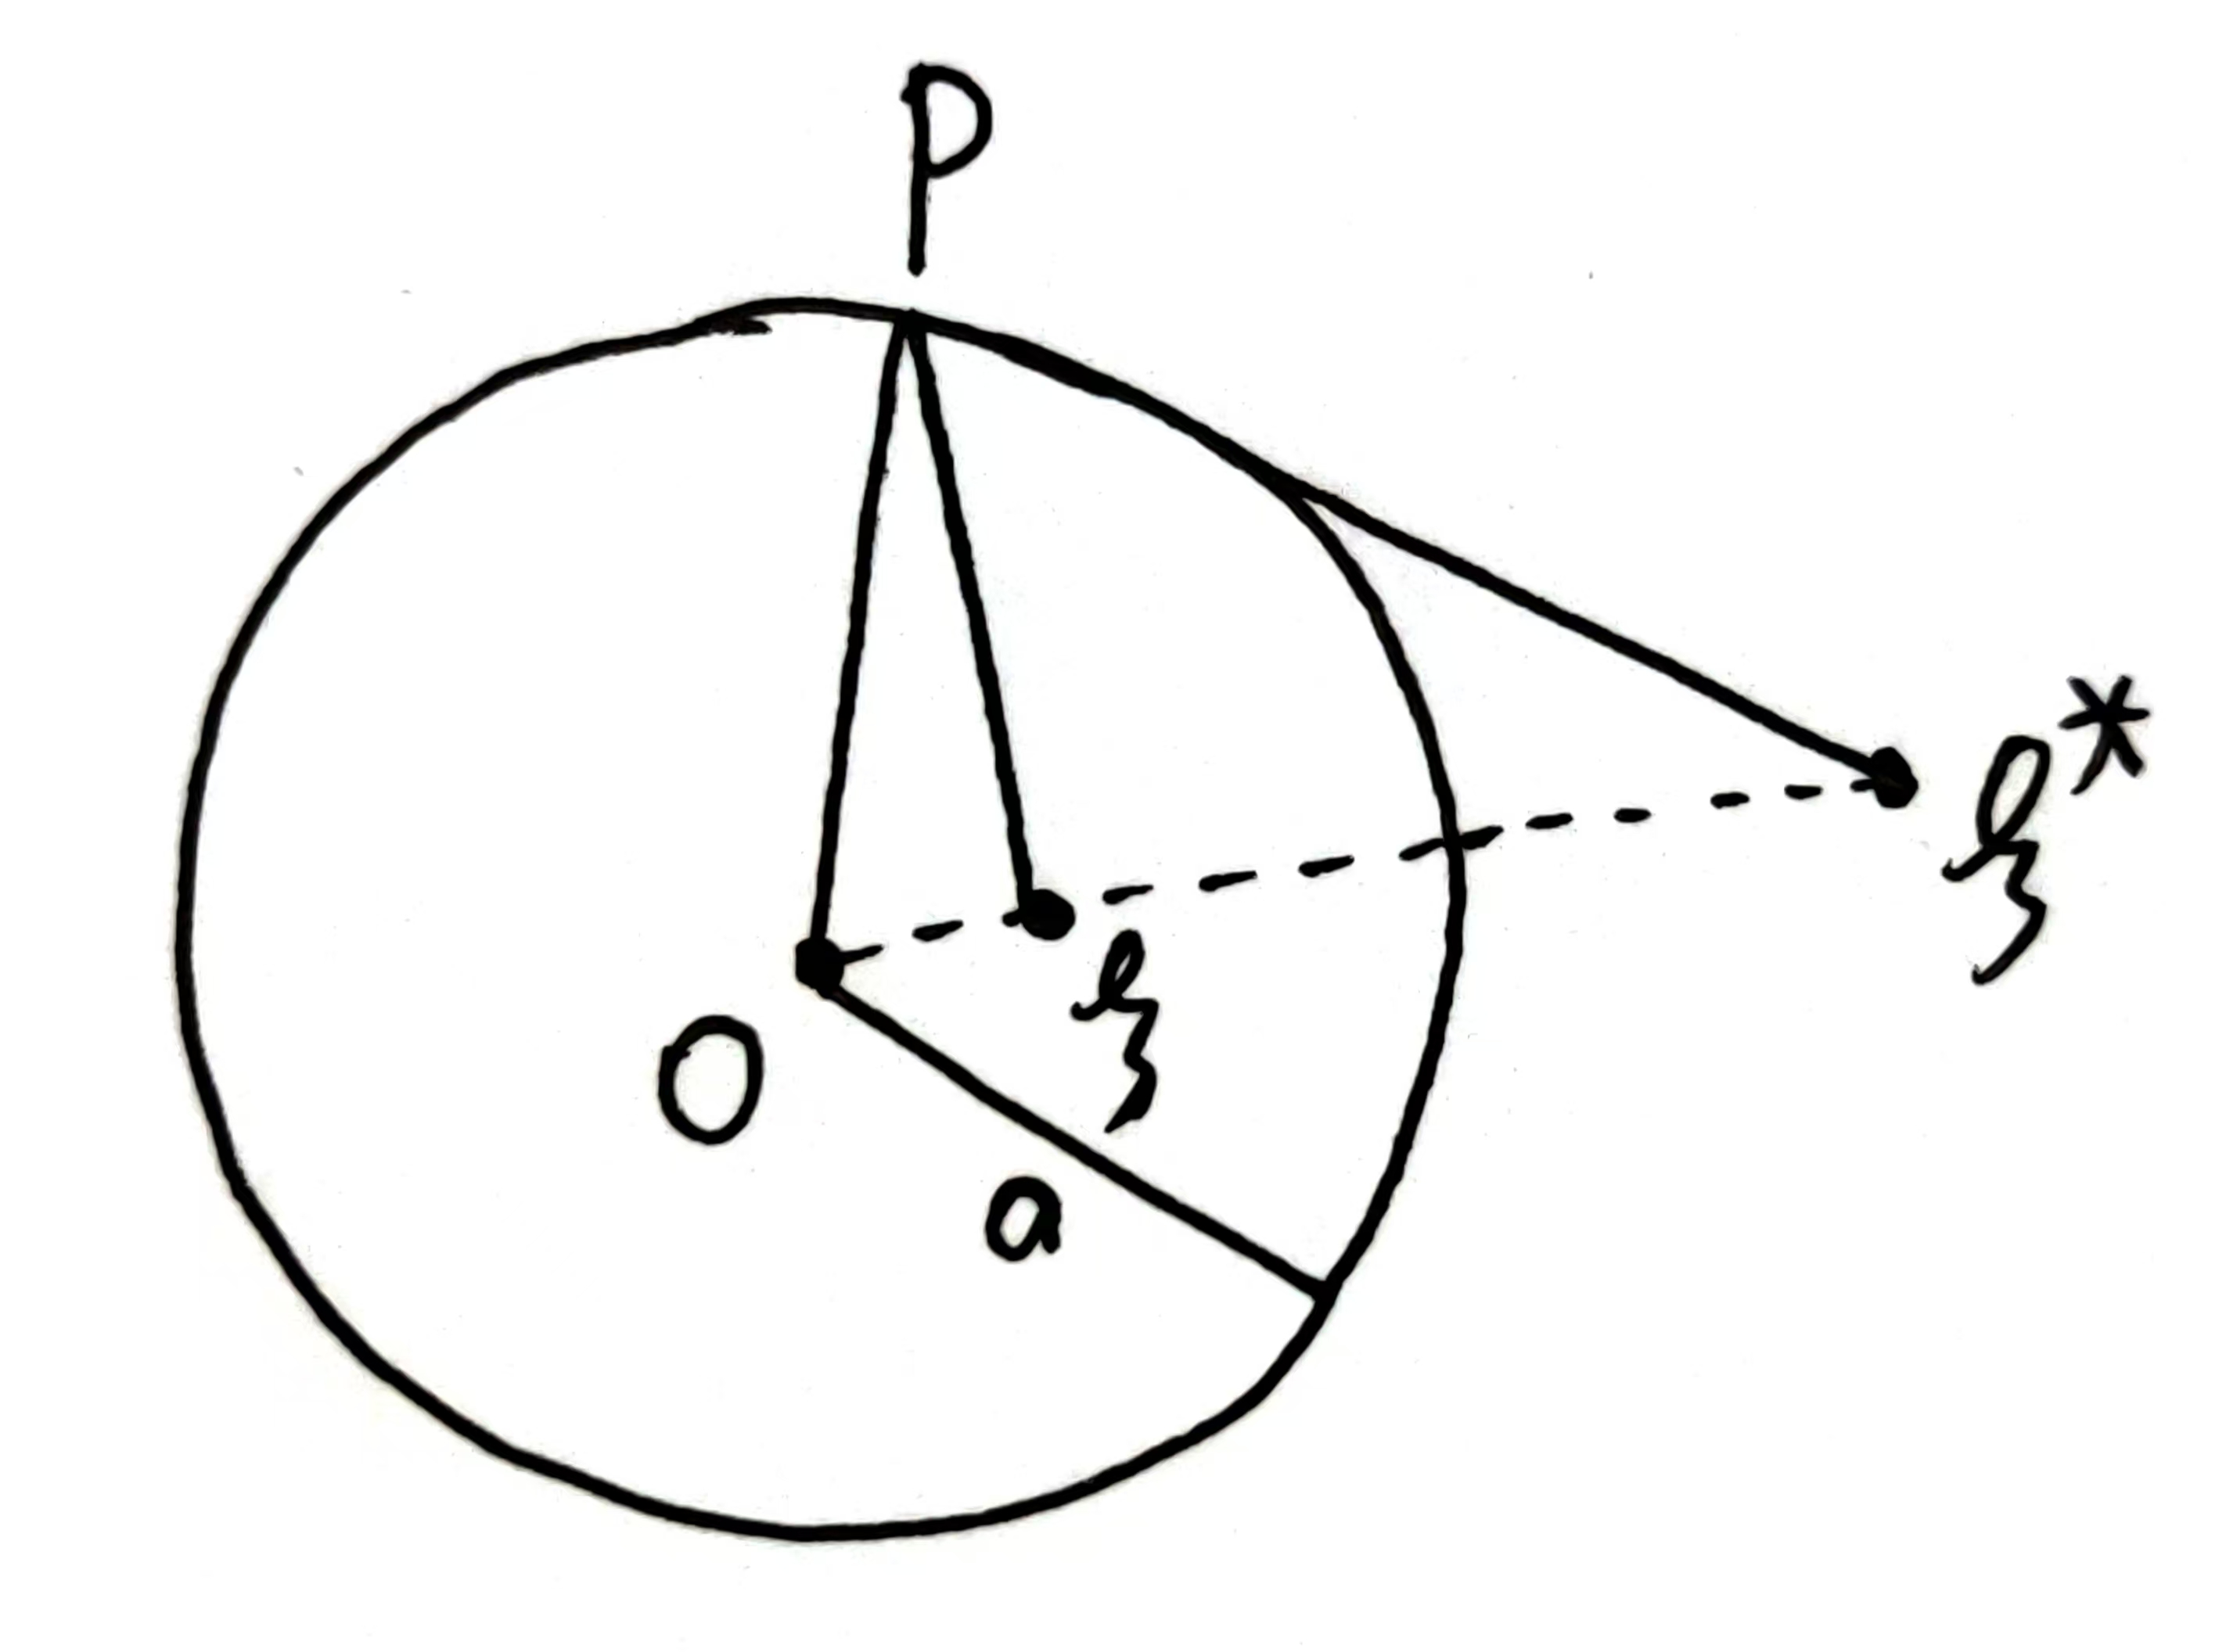
\includegraphics[width=0.3\linewidth]{figure/3.5-1}
					\caption{球$\Omega = B_a$ 及$O, \xi , \xi^*$ 点}
					\label{pic : 3.5-1} % 添加图像引用标签
				\end{figure}
				
				则根据三角形的相似关系 ($\triangle D \xi P \sim \triangle DP\xi^*$), 可得到
				\begin{align*}
					\begin{dcases*}
						| \xi | \cdot | \xi^* | = a^2 \\
						\frac{| P\xi |}{| P \xi^* |} = \frac{| \xi |}{a} , \,\, \forall P \in \partial B_a
					\end{dcases*} 
					\,\,\,\, \Rightarrow \,\,\,\, 
					\begin{dcases*}
						K(x , \xi) = C \cdot | x - \xi |^{2 - n} \\
						K(x , \xi^*) = C \cdot | x - \xi^* |^{2 - n} \\
						\frac{K(x , \xi)}{K(x , \xi^*)} 
						= \frac{| x - \xi|^{2 - n}}{| x - \xi^* |^{2 - n}} 
						= \left( \frac{| \xi |}{a} \right)^{2 - n} , \,\, \forall x \in \partial B_a
					\end{dcases*}
				\end{align*}
				where $C = \dfrac{1}{(2 - n) w_n}$ constant. Let
				\[ v(x , \xi) = -\left( \dfrac{| \xi |}{a} \right)^{2 - n} K(x , \xi^*) \]
				Then $v$ satisfies
				\begin{align*}
					\begin{dcases*}
						\Delta v = 0 \,\, \text{on} \,\, \Omega \\
						v = -K(x , \xi) \,\, \text{on} \,\, \partial \Omega
					\end{dcases*}
				\end{align*}
				于是$v(x , \xi)$ 存在, 从而Green's Function存在, i.e. 
				\begin{align*}
					G(x , \xi) 
					= K(x , \xi) + v(x , \xi) 
					= C \cdot \left( | x - \xi |^{2 - n} - \left( \dfrac{| \xi |}{a} \right)^{2 - n} \cdot \left| x - \left( \frac{a}{| \xi |} \right)^2 \xi \right|^{2 - n} \right)
				\end{align*}
				下面来给出Poisson公式, 即计算$\dfrac{\partial G(x , \xi)}{\partial n_x}$ on $\partial B_a$:
				
				\newpage
				
				\begin{align*}
					\left. \frac{\partial G}{\partial n} \right|_{| x | = a} 
					&= \sum_{i = 1}^n \frac{\partial G}{\partial x_i} \cdot \left. \frac{\partial x_i}{\partial n} \right|_{| x | = a} \\
					&= \sum_{i = 1}^n \frac{Cx_i}{a} 
					\left( (2 - n) \cdot |x - \xi|^{1 - n} \cdot \frac{x_i - \xi_i}{| x - \xi |} - (2 - n) \cdot \left( \dfrac{| \xi |}{a} \right)^{2 - n} \cdot  \left| x - \left( \frac{a}{| \xi |} \right)^2 \xi \right|^{1 - n} \cdot \frac{x_i - \left( \dfrac{a}{| \xi |} \right)^2 \xi_i}{\left| x - \left( \dfrac{a}{| \xi |} \right)^2 \xi \right|} \right) \\
					&= \sum_{i = 1}^n \frac{x_i}{a w_n} 
					\left( | x - \xi |^{-n} (x_i - \xi_i) - \left( \frac{| \xi |}{a} \right)^{2 - n} \cdot \left| x - \left( \frac{a}{| \xi |} \right)^2 \xi \right|^{-n} \cdot \left( x_i - \left( \frac{a}{| \xi |} \right)^2 \xi_i \right) \right) \\
					&= \frac{1}{a w_n} 
					\left( | x - \xi |^{-n} \cdot \Big( | a |^2 - \overrightarrow{x} \cdot \overrightarrow{\xi} \Big) - \left( \frac{| \xi |}{a} \right)^{2 - n} \cdot \left| x - \left( \frac{a}{| \xi |} \right)^2 \xi \right|^{-n} \cdot \left( a^2 - \left( \frac{a}{| \xi |} \right)^2 \overrightarrow{x} \cdot \overrightarrow{\xi} \right) \right)
				\end{align*}
				此时关注\uwave{$\overrightarrow{x} \cdot \overrightarrow{\xi}$}项, 其系数为:
				\begin{align*}
					\left( \frac{| \xi |}{a} \right)^{-n} \cdot \left| x - \left( \frac{a}{| \xi |} \right)^2 \xi \right|^{-n} - | x - \xi |^{-n}
				\end{align*}
				由几何关系可知, $\forall x \in \partial B_a$, $\forall \xi \in B_a$, $\st$
				\begin{align*}
					 \left| \left( \frac{| \xi |}{a} \right) x - \left( \frac{a}{| \xi |} \right) \xi \right|  
					= | x - \xi |
				\end{align*}
				
				\begin{figure}[thbp!]
					\centering
					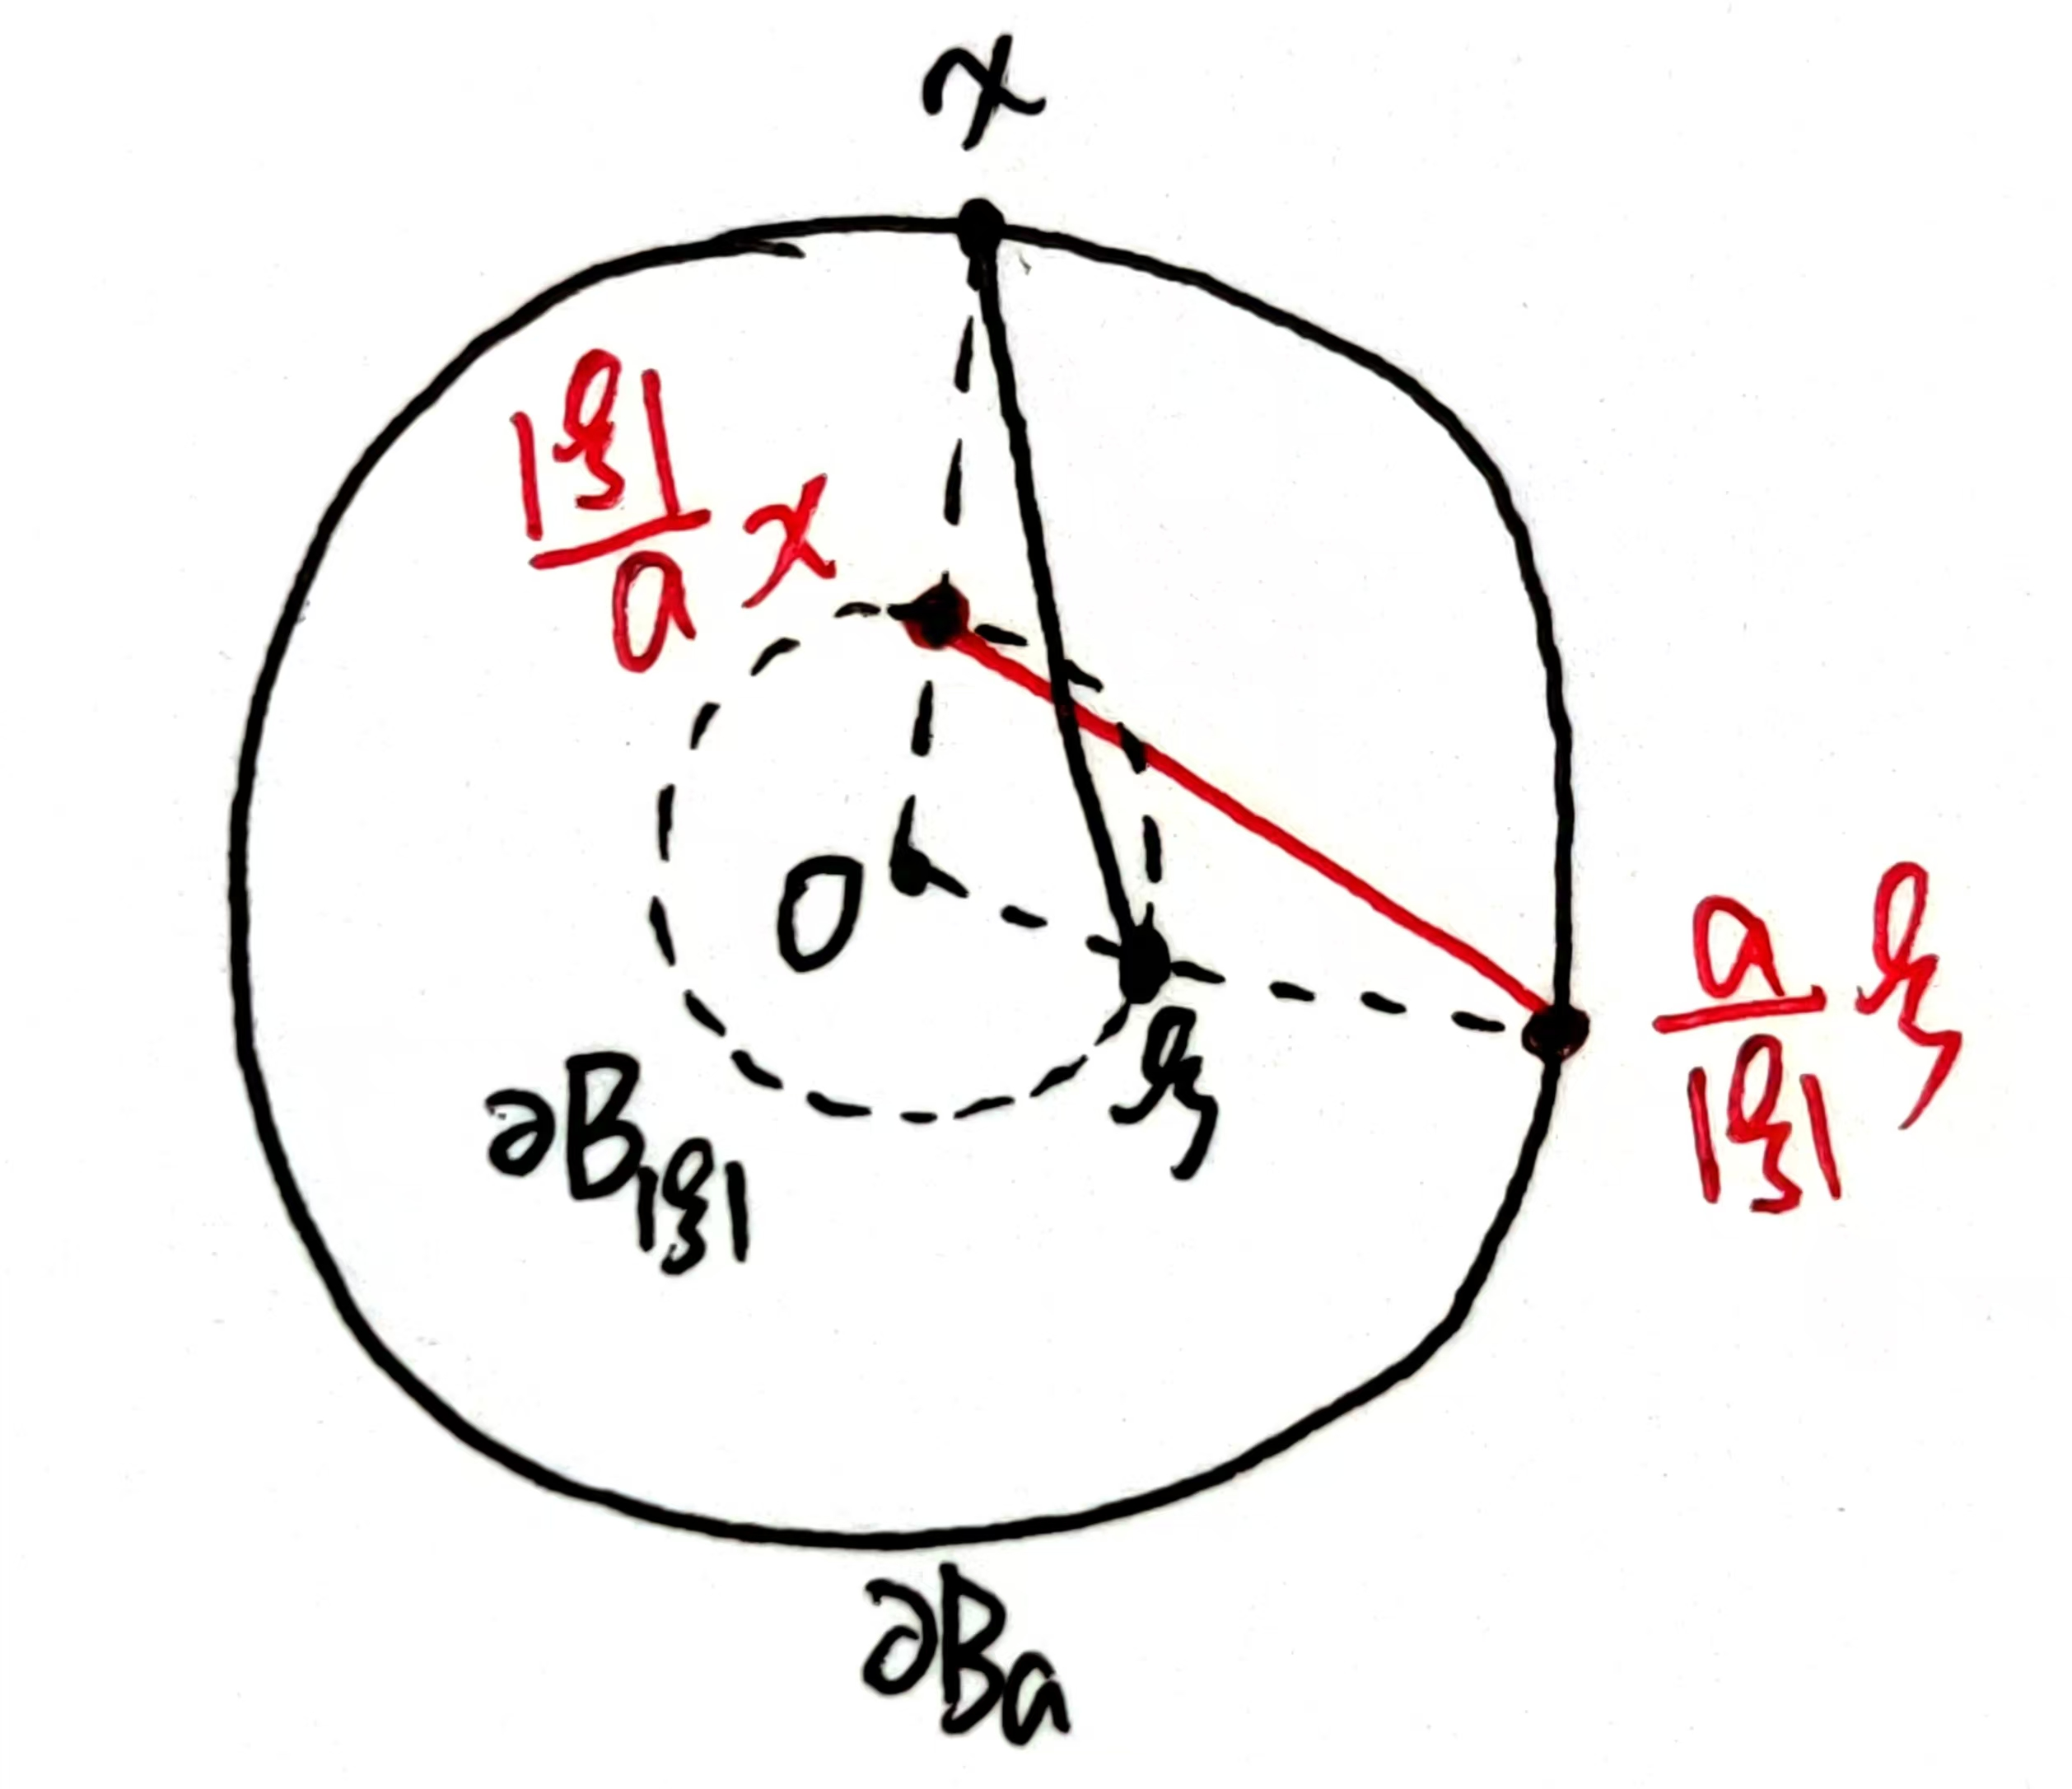
\includegraphics[width=0.27\linewidth]{figure/3.5-2}
					\caption{$\left| \left( \dfrac{| \xi |}{a} \right) x - \left( \dfrac{a}{| \xi |} \right) \xi \right| = | x - \xi |$}
					\label{pic : 3.5-2} % 添加图像引用标签
				\end{figure}
				
				故\uwave{$\overrightarrow{x} \cdot \overrightarrow{\xi}$}项系数:
				\begin{align*}
					\left( \frac{| \xi |}{a} \right)^{-n} \cdot \left| x - \left( \frac{a}{| \xi |} \right)^2 \xi \right|^{-n} - | x - \xi |^{-n} 
					= 0
				\end{align*}
				从而
				\begin{align*}
					\left. \frac{\partial G}{\partial n} \right|_{| x | = a} 
					&= \frac{a^2}{a w_n} \left[ | x - \xi |^{-n} - \left( \frac{| \xi |}{a} \right)^2 | x - \xi |^{-n} \right] \\
					&= \frac{a}{w_n} \left( 1 - \frac{| \xi |^2}{a^2} \right) \cdot | x - \xi |^{-n} 
					= \frac{a^2 - | \xi |^2}{a w_n | x - \xi |^n}
				\end{align*}
				根据\textbf{Def \ref{def 3.5.1} 式(\ref{3.3})}, $\forall u \in C^2(\Omega) \cap C^1 \left(	\overline{\Omega} \right)$, 若$u$ 为齐次Dirichlet Problem的解, 则必有
				\begin{align*}
					u(\xi) 
					= \int_{\partial B_a} \frac{a^2 - | \xi |^2}{a w_n | x - \xi |^n} \, f(x) \, dS_x , \,\, \forall \xi \in B_a
				\end{align*}
			
				\newpage
				
				\item[\underline{\textbf{Step 2}}]:\underline{\textbf{证明$u$ in (\ref{3.4}) $\in C^2(\Omega)$}}:
				
				\vspace*{1em}
				
				由于$\dfrac{a^2 - | \xi |^2}{a w_n | x - \xi |^n}, \,\, x \in \partial B_a$ 为关于$\xi$ 的初等函数, 因此$u \in C^2(\Omega)$. 
				
				\vspace*{4em}
				
				\item[\underline{\textbf{Step 3}}]:\underline{\textbf{证明$\Delta u = 0$ on $B_a$}}:
				\begin{align*}
					\Delta u 
					= \Delta_\xi \int_{\partial B_a} \frac{a^2 - | \xi |^2}{a w_n | x - \xi |^n} f(x) \, dS_x 
					= \int_{\partial B_a} \Delta \left( \frac{a^2 - | \xi |^2}{a w_n | x - \xi |^n} \right) f(x) \, dS_x
				\end{align*}
				Since 
				\begin{align*}
					\partial_{\xi_i} \left( \frac{a^2 - | \xi |^2}{| x - \xi |^n} \right)
					= \frac{-2\xi_i}{| x - \xi |^n} + \frac{n \Big( a^2 - | \xi |^2 \Big)}{| x - \xi |^{n + 2}} (x_i - \xi_i) , \,\, \forall i = 1 \sim n
				\end{align*}
				Then (计算过程过于繁琐, 此处省略)
				\begin{align*}
					\Delta \left( \frac{a^2 - | \xi |^2}{| x - \xi |^n} \right) 
					= 0
				\end{align*}
				Thus $\Delta u = 0$. 
				
				\vspace*{4em}
				
				\item[\underline{\textbf{Step 4}}]:\underline{\textbf{证明$u \in C^0(\partial \Omega)$ 且$u = f$ on $\partial \Omega$}}, 即证极限
				\begin{align*}
					\lim_{\substack{\xi \to \bar{x} \\ \xi \in B_a}} u(\xi) = f(\bar{x}) , \,\, \forall \bar{x} \in \partial B_a
				\end{align*}
				WTS:$\forall \varepsilon > 0$, $\exists \delta > 0$, $\st$
				\begin{align*}
					\left| \int_{\partial B_a} \frac{a^2 - | \xi |^2}{a w_n | x - \xi |^n} \, f(x) \, dS_x - f(\bar{x}) \right| < \varepsilon , \,\, \forall | \bar{x} - \xi | < \delta , \,\, \xi \in B_a
				\end{align*}
				注意到\footnote{当$f \equiv 1$ 时, 对于方程
					$\begin{dcases*}
						\Delta u = 0 \,\, B_a \\
						u = 1 \,\, \partial B_a
					\end{dcases*}$
					, 根据\textbf{Step 1} 讨论, 若有解则其解一定具有形式
					\[ u(\xi) = \int_{\partial B_a} \frac{a^2 - | \xi |^2}{a w_n | x - \xi |^n} \, dS_x \]
					而对此Dirichlet Problem, 不难发现$u \equiv 1$ 为一个解. 因此根据\textbf{Dirichlet问题解的唯一性 (Prop \ref{prop 3.4.2})}, 该积分$\equiv 1$. }
				\begin{align*}
					\int_{\partial B_a} \frac{a^2 - | \xi |^2}{a w_n | x - \xi |^n} \, dS_x \equiv 1 , \,\, \forall \xi \in B_a
				\end{align*}
				即证
				\begin{align*}
					\left| \int_{\partial B_a} \frac{a^2 - | \xi |^2}{a w_n | x - \xi |^n} \, \Big( f(x) - f(\bar{x}) \Big) \, dS_x \right| < \varepsilon , \,\, \forall | \bar{x} - \xi | < \delta , \,\, \xi \in B_a
				\end{align*}
				
				\newpage
				\begin{align*}
					\int_{\partial B_a} \sim 
					= \int_{\partial B_a \backslash B_{\delta_1}(\bar{x})} \sim + \int_{\partial B_a \cap B_{\delta_1}(\bar{x})} \sim
				\end{align*}
				下面分为两个部分逐次讨论:
				
				\vspace*{1em}
				
				\begin{enumerate}
					\item[\underline{\textbf{$1^{\circ}$}}]:Since $f \in C(\partial B_a)$, then $\exists \delta_1 > 0$, $\st$
					\begin{align*}
						| f(x) - f(\bar{x}) | < \frac{\varepsilon}{2} , \,\, \forall | x - \bar{x} | < \delta_1
					\end{align*}
					于是
					\begin{align*}
						\left| \int_{\partial B_a \cap B_{\delta_1}(\bar{x})} \sim \right| 
						\leq \frac{\varepsilon}{2} \cdot \left| \int_{\partial B_a \cap B_{\delta_1}(\bar{x})} \frac{a^2 - | \xi |^2}{a w_n | x - \xi |^n} \, dS_x \right| 
						\leq \frac{\varepsilon}{2} \cdot \left| \int_{\partial B_a} \frac{a^2 - | \xi |^2}{a w_n | x - \xi |^n} \, dS_x \right| = \frac{\varepsilon}{2}
					\end{align*}
					
					\vspace*{4em}
					
					\item[\underline{\textbf{$2^{\circ}$}}]:Set $\delta \leq \dfrac{\delta_1}{2}$, then 对于积分区域中的$x$, 
					\begin{align*}
						x \in \partial B_a \backslash B_{\delta_1}(\bar{x}) \,\, \& \,\, | \bar{x} - \xi | < \delta \leq \frac{\delta_1}{2} \hspace{2em} \Rightarrow \hspace{2em} | x - \xi | \geq \frac{\delta_1}{2}
					\end{align*}
					
					\begin{figure}[thbp!]
						\centering
						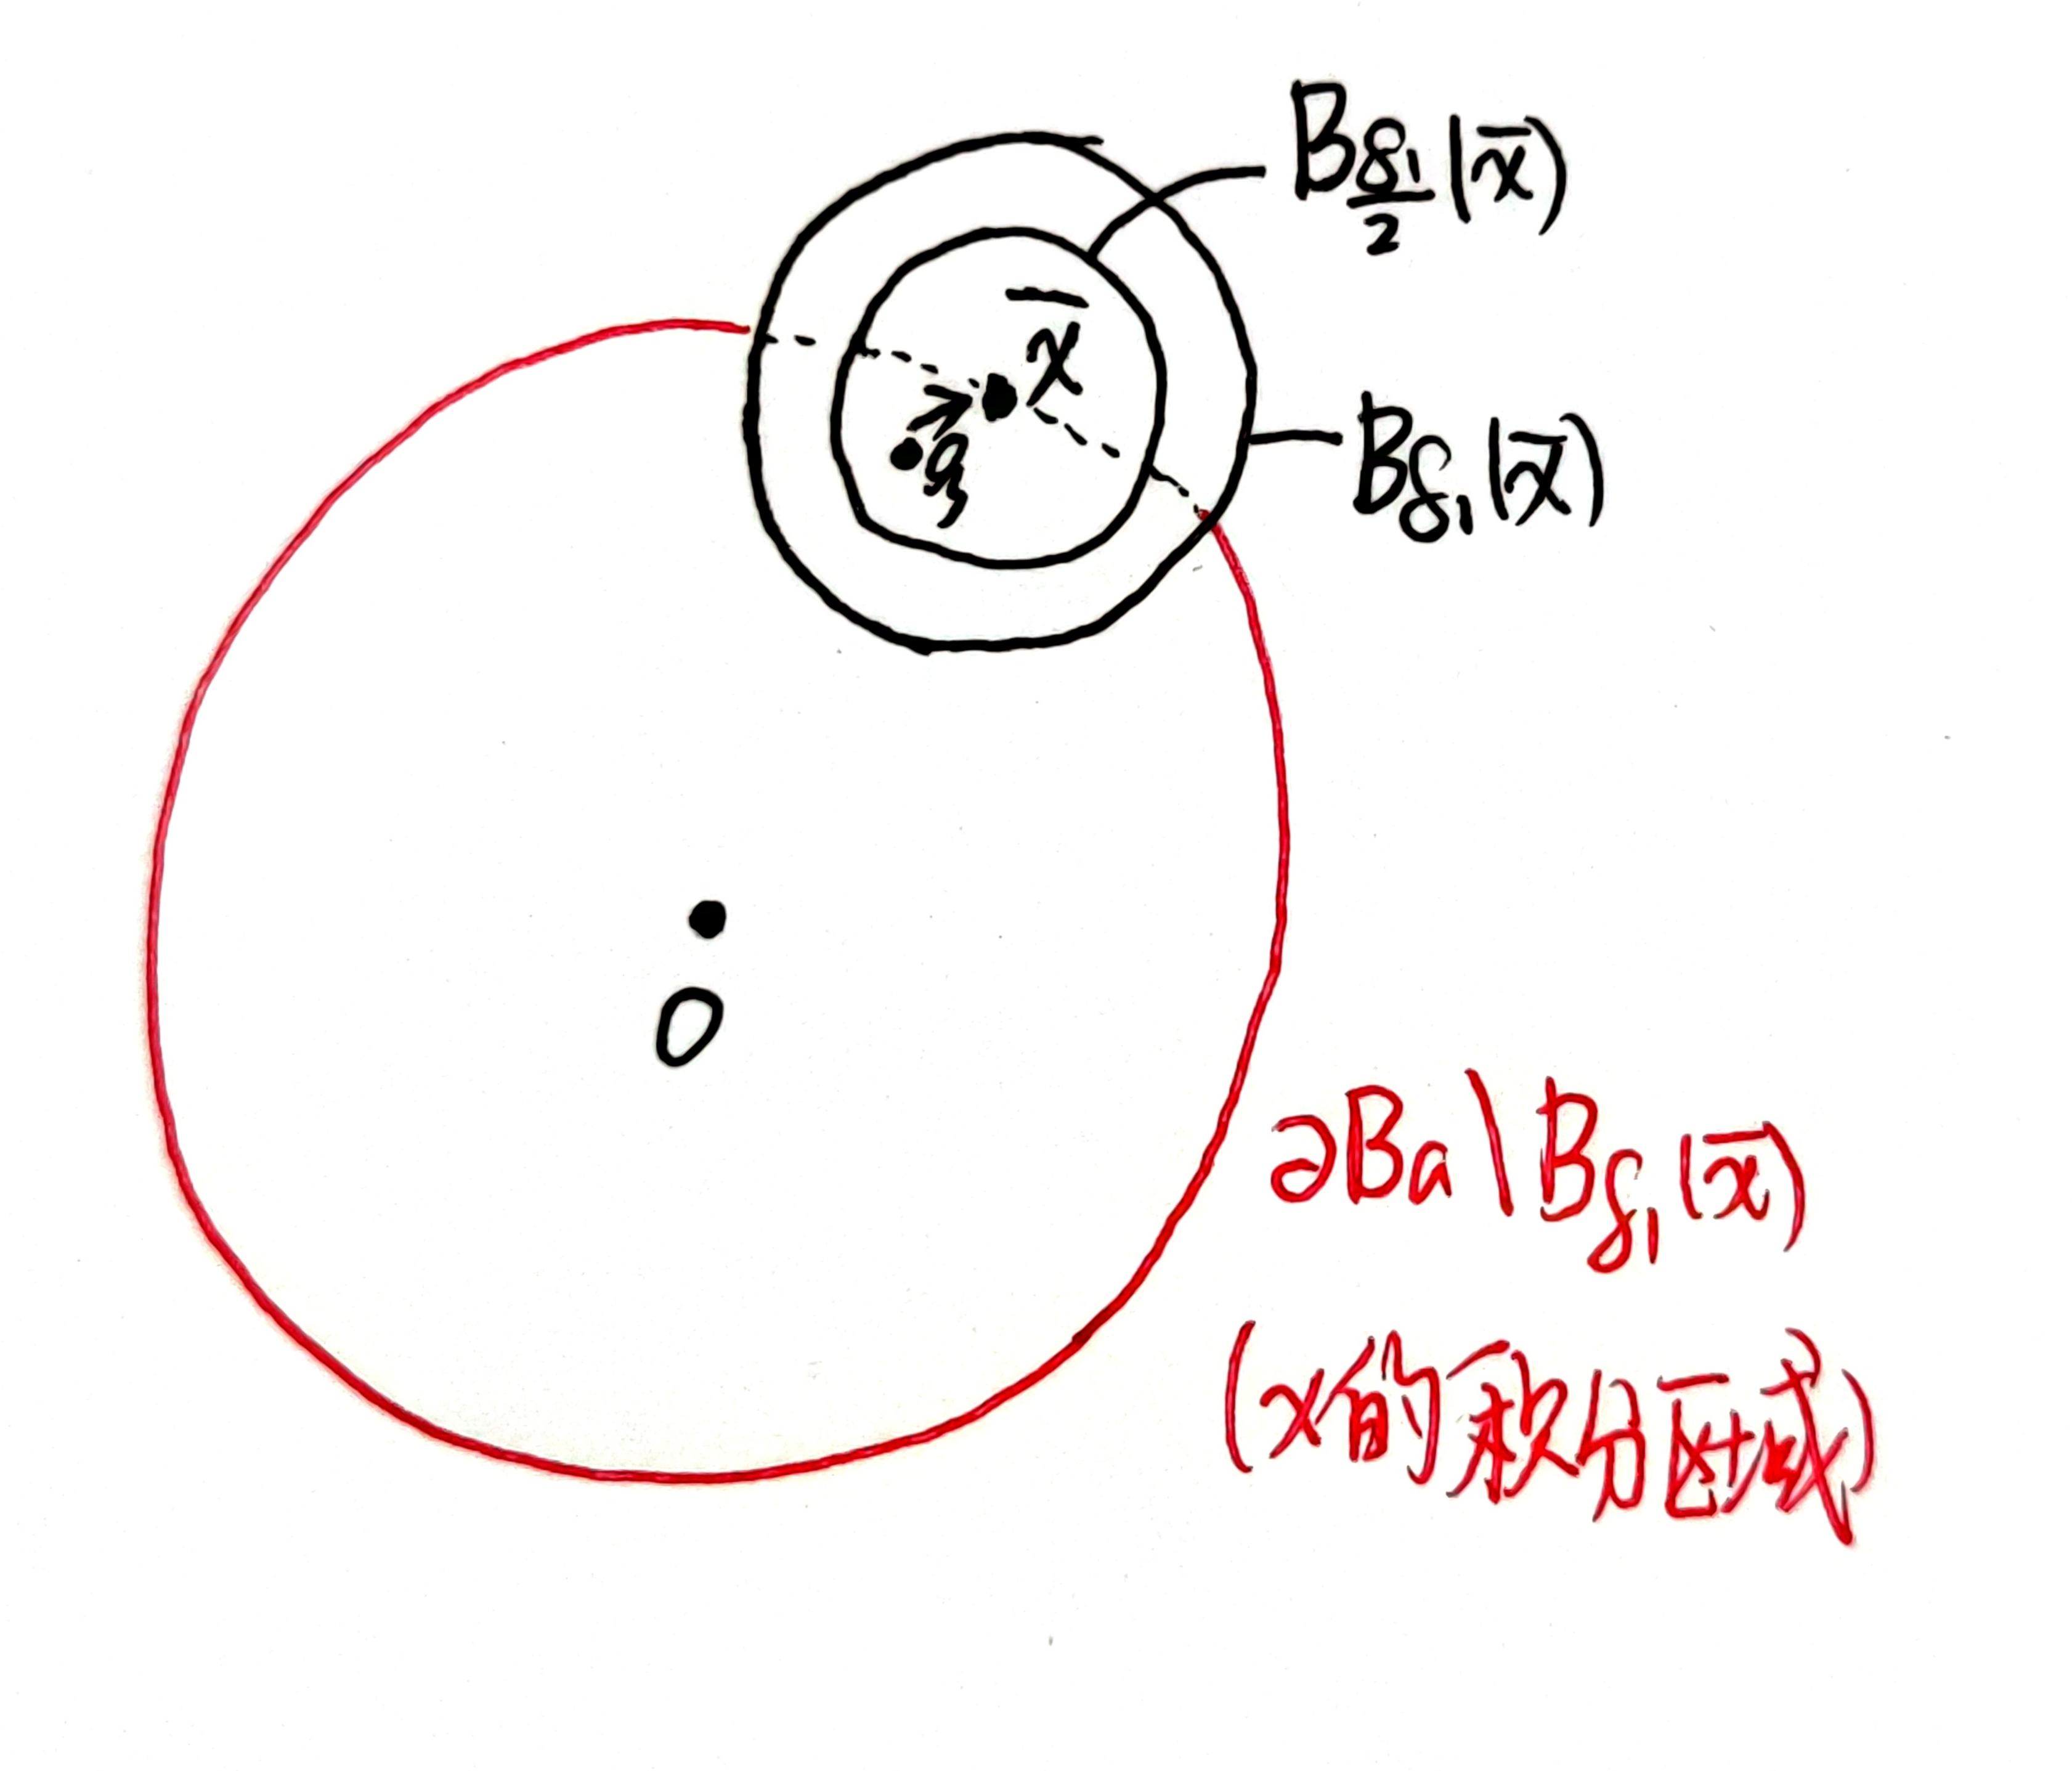
\includegraphics[width=0.3\linewidth]{figure/3.5-3}
						\caption{$x$ 的积分区域及$x , \xi , \bar{x}$ 的位置关系}
						\label{pic : 3.5-3} % 添加图像引用标签
					\end{figure}
					
					Since $f \in C(\partial B_a)$, then $\exists M > 0$, $\st | f | \leq M$ on $\partial B_a$. \\
					Hence
					\begin{align*}
						\left| \int_{\partial B_a \backslash B_{\delta_1}(\bar{x})} \sim \right| 
						&\leq \int_{\partial B_a \backslash B_{\delta_1}(\bar{x})} \frac{\Big( a^2 - | \xi |^2 \Big) \cdot \Big( \left| f(x) \right| + \left| f(\bar{x}) \right| \Big)}{a w_n \cdot \left( \dfrac{\delta_1}{2} \right)^n} \, dS_x \\
						&\leq \int_{\partial B_a \backslash B_{\delta_1}(\bar{x})} \frac{2M \cdot \Big( a^2 - | \xi |^2 \Big) }{a w_n \cdot \left( \dfrac{\delta_1}{2} \right)^n} \, dS_x 
					\end{align*}
					
					\newpage
					
					由于$\xi \to \bar{x}$ 过程中, $| \xi | \to a$, 因此we can take $\delta_2 > 0$, $\st$ 
					\begin{align*}
						a^2 - | \xi |^2 
						\leq \frac{a w_n \cdot \left( \dfrac{\delta_1}{2} \right)^2}{2M} \cdot \frac{1}{| \partial B_a |} \cdot \frac{\varepsilon}{2} , \,\, \forall | \bar{x} - \xi | < \delta_2
					\end{align*}
					Let $\delta = \min \{ \dfrac{\delta_1}{2} , \delta_2 \} > 0$, then
					\begin{align*}
						\left| \int_{\partial B_a \backslash B_{\delta_1}(\bar{x})} \sim \right| 
						&\leq \int_{\partial B_a \backslash B_{\delta_1}(\bar{x})} \frac{2M \cdot \Big( a^2 - | \xi |^2 \Big) }{a w_n \cdot \left( \dfrac{\delta_1}{2} \right)^n} \, dS_x \\
						&\leq \frac{\varepsilon}{2} \cdot \frac{1}{| \partial B_a |} \cdot \int_{\partial B_a \backslash B_{\delta_1}(\bar{x})} 1 \, dS_x \\
						&\leq \frac{\varepsilon}{2} , \,\, \forall | \bar{x} - \xi | < \delta
					\end{align*}
				\end{enumerate}
				
				\vspace*{2em}
				
				\hspace{-1.95em}综上所述, for any fixed $x \in \partial B_a$, $\forall \varepsilon > 0$, $\exists \delta_1 , \delta > 0$, $\st$
				\begin{align*}
					\left| u(\xi) - f(\bar{x}) \right| 
					&= \left| \int_{\partial B_a} \frac{a^2 - | \xi |^2}{a w_n | x - \xi |^n} \, \Big( f(x) - f(\bar{x}) \Big) \, dS_x \right| \\
					&\leq \int_{\partial B_a \backslash B_{\delta_1}(\bar{x})} \sim + \int_{\partial B_a \cap B_{\delta_1}(\bar{x})} \sim \\
					&\leq \frac{\varepsilon}{2} + \frac{\varepsilon}{2} 
					= \varepsilon , \,\, \forall | \bar{x} - \xi | < \delta
				\end{align*}
				Therefore, 
				\begin{align*}
					\lim_{\substack{\xi \to \bar{x} \\ \xi \in B_a}} u(\xi) = f(\bar{x}) , \,\, \forall \bar{x} \in \partial B_a
				\end{align*}
				i.e. $u = f$ on $\partial B_a$ and $u \in C^0\left( \partial B_a \right)$. 
			\end{enumerate}
		\end{proof}
	\end{thm}

\newpage

\section{Perron's Method (一般有界区域上求解Dirichlet问题)}
	这一节我们将给出\textbf{一般区域上Dirichlet Problem的构造性求解}. 在此之前, 我们先来做一些准备工作, 重新定义\textbf{下调和函数}, 并给出其相关性质. 
	
\vspace*{2em}

\subsection{下调和函数的定义}
	首先我们在此前$\S 3.4$ 节粗略定义\underline{\textbf{“$\Delta u \geq 0$”}}的基础上, 给出下调和函数更广泛的定义. 
	
	\vspace*{1em}
	
	\begin{defn}\label{def 3.6.1}
		设$u \in C \left( \overline{\Omega} \right)$. 若
		\begin{align*}
			u(\xi) \leq \fint_{\partial B_{\rho}(\xi)} u(x) \, dS_x , \,\, \forall \overline{B_{\rho}(\xi)} \subset \Omega \,\, \text{for $\rho$ small}
		\end{align*}
		则称$u$ \underline{\textcolor{blue}{\textbf{下调和 (subharmonic)}}}, 记为$u \in \sigma(\Omega)$. 
		
		\vspace*{4em}
		
		\begin{rmk}
			\begin{itemize}
				\item 下调和的条件的含义是指对于$\forall$ fixed $\xi \in \Omega$, 都存在与$\xi$ 有关的半径$r > 0$, $\st$
				\begin{align*}
					u(\xi) \leq \fint_{\partial B_{\rho}(\xi)} u(x) \, dS_x , \,\, \forall \rho \leq r , \,\, \text{where} \,\, \overline{B_{r}(\xi)} \subset \Omega
				\end{align*}
				
				\vspace*{4em}
				
				\item 该定义事实上为\underline{“$\Delta u \geq 0$”}的推广, 即若$u \in \sigma(\Omega) \cap C^2(\Omega)$, 则$\Delta u \geq 0$. 
				
				\vspace*{2em}
				
				\begin{proof}
					$\forall \xi \in \Omega$, $\exists r > 0$, $\st$
					\begin{align*}
						u(\xi) \leq \fint_{\partial B_{\rho}(\xi)} u(x) \, dS_x , \,\, \forall \rho \leq r
					\end{align*}
					对半径积分可得球体上的均值不等式
					\begin{align*}
						u(\xi) \leq \fint_{B_{\rho}(\xi)} u(x) \, dS_x , \,\, \forall \rho \leq r
					\end{align*}
					由于$u$ 在$\xi$ 点连续, 因此$\exists \rho_0 < r$, $\st$
					\begin{align*}
						u(x) \geq u(\xi) , \,\, \forall x \in B_{\rho_0}(\xi)
					\end{align*}
					即$\xi$ 为局部极小点, $\Delta u \geq 0$. 
				\end{proof}
			\end{itemize}
		\end{rmk}
	\end{defn}

\newpage

\subsection{极值原理 (Maximum Principle)}
	与$\S 3.4$ 节中讨论类似, 对于推广形式的下调和函数, 其也有\textbf{极值原理} (对应\textbf{Thm \ref{thm 3.4.4} 强极值原理}). 
	
	\vspace*{1em}
	
	\begin{thm}\label{thm 3.6.1}
		\textbf{[下调和函数的极值原理 (Maximum Principle)]}. \\
		Suppose $\Omega$ bounded and connected, $u \in \sigma(\Omega)$. Then 
		\begin{align*}
			\max_{\overline{\Omega}} u = \max_{\partial \Omega} u
		\end{align*}
		
		\vspace*{1em}
		
		\begin{proof}
			类比\textbf{Thm \ref{thm 3.4.4}}证明. 
		\end{proof}
	\end{thm}

\vspace*{3.5em}

\subsection{比较原理 (Comparision Principle)}
	下面我们将说明, 对于下调和函数$u$, 若其在边界$\partial \Omega$ 上能被调和函数$v$控制, 则其在整个区域$\overline{\Omega}$ 上均能被$v$ 控制. 这就是所谓的\textbf{比较原理 (Comparision Principle)}. 
	
	\vspace*{1em}
	
	\begin{thm}\label{thm 3.6.2}
		\textbf{[下调和函数的比较原理 (Comparision Principle)]}. \\
		Suppose $u \in \sigma(\Omega)$, $v \in C^2(\Omega) \cap C \left( \overline{\Omega} \right)$, 且$\Delta v = 0$ on $\Omega$. If
		\begin{align*}
			u \Big|_{\partial \Omega} \leq v \Big|_{\partial \Omega}
		\end{align*}
		Then $u \leq v$ on $\overline{\Omega}$. 
		
		\vspace*{1em}
		
		\begin{proof}
			不难得到$u - v \in \sigma(\Omega)$ 下调和, 利用\textbf{下调和函数极值原理 (Thm \ref{thm 3.6.1})} 即可得证. 
		\end{proof}
	\end{thm}

\vspace*{3em}

\subsection{最大值max函数保持下调和}
	
	\begin{proposition}\label{prop 3.6.1}
		\textbf{[最大值max函数保持下调和]}. \\
		Suppose $u_1 , u_2 \in \sigma(\Omega)$, then 
		\begin{align*}
			\overline{u}(x) = \max \{ u_1(x) , u_2(x) \} \in \sigma(\Omega)
		\end{align*}
		
		\begin{rmk}
			利用定义即证. 事实上可拓展至任意有限个函数的最大值, 即
			\[ u_1 , \cdots , u_n \in \sigma(\Omega) \,\, \Rightarrow \,\, \max\{ u_1 , \cdots , u_n \} \in \sigma(\Omega) \] 
		\end{rmk}
	\end{proposition}

\newpage

\subsection{一致有界调和函数列有一致收敛子列}
	下面我们将说明, 对于一致有界的调和函数列, 其在调和区域$\Omega$ 的任一\textbf{紧包含\footnote{若区域$\overline{\Omega^{'}} \subset \Omega$, 则称$\Omega^{'}$ \underline{\textcolor{blue}{\textbf{紧包含于}}} $\Omega$, 记为$\Omega^{'} \subset\subset \Omega$. }}区域$\Omega^{'}$ 上都存在一致收敛的子列. 事实上可视作泛函分析中\textbf{Arzel\`{a}-Ascoli定理}的应用. 
	
	\vspace*{1em}
	
	\begin{thm}\label{thm 3.6.3}
		\textbf{[一致有界调和函数列有一致收敛子列]}. \\
		Suppose $\{ u_n \}_{n = 1}^{\infty} \subset C^2(\Omega) \cap C \left( \overline{\Omega} \right)$, $\Delta u_n = 0$, $\forall n \in \N$. If $\{ u_n \}_{n = 1}^{\infty}$ uniformly bounded, then \\
		对于$\forall \Omega^{'} \subset \subset \Omega$, $\exists \{ u_{n_k} \}_{k = 1}^{\infty} \subset \{ u_n \}_{n = 1}^{\infty}$, $\st$ 
		\begin{align*}
			u_{n_k} \rightrightarrows \overline{u} \,\, \text{uniformly in} \,\, \Omega^{'} \subset\subset \Omega, \,\, \text{且} \,\, \Delta \overline{u} = 0 \,\, \text{on} \,\, \Omega^{'} 
		\end{align*} 
		
		\vspace*{4em}
		
		\begin{proof}
			设$| u_n | \leq M , \,\, \forall n \in \N$ on $\overline{\Omega}$. 对于$\{ u_n \}_{n = 1}^\infty$ 中任意一项$u$. 由于$u \in C^2(\Omega)$ 且$\Delta u = 0$, \\
			因此根据\textbf{Prop \ref{prop 3.2.1}}, $u \in C^{\infty}(\Omega)$, 各阶导数存在 $\,\, \Rightarrow \,\, \Delta u_{x_i} = 0 , \,\, \forall i = 1 \sim n$. \\
			根据\textbf{调和函数平均值等式 (Cor \ref{cor 3.4.1})}及\textbf{Gauss-Green公式 (Thm \ref{thm B.4.1} (\rmnum{1}))}, 
			\begin{align*}
				u_{x_i}(\xi) 
				= \frac{1}{| B_\rho |} \int_{B_{\rho}(\xi)} u_{x_i}(x) \, dx 
				= \frac{1}{| B_\rho |} \int_{\partial B_{\rho}(\xi)} u \cdot n_i \, dS_x , \,\, \forall \overline{B_{\rho}(\xi)} \subset \Omega
			\end{align*}
			由于$| u | \leq M$ on $\overline{\Omega}$, 因此
			\begin{align*}
				| u_{x_i} (\xi) | 
				\leq \frac{1}{| B_\rho |} \int_{\partial B_\rho(\xi)} M \, dS_x 
				= \frac{n M}{\rho} , \,\, \forall \overline{B_{\rho}(\xi)} \subset \Omega
			\end{align*}
			由于$\Omega^{'} \subset\subset \Omega$, 因此可取$\rho = d(\partial \Omega , \partial \Omega^{'}) > 0$, 从而$\{ u_n \}_{n = 1}^{\infty}$ 的各阶导数一致有界. \\
			$\Rightarrow \,\, \{ u_n \}_{n = 1}^{\infty}$ 等度连续 $\,\, \Rightarrow \,\,$ 根据\textbf{Arzel\`{a}-Ascoli定理\footnote{详见\textbf{《泛函分析--自学笔记》 Thm 1.8.1}. }}, $\{ u_n \}_{n = 1}^{\infty}$ 在$\Omega^{'}$ 上一致收敛. 记
			\begin{align*}
				u_{n_k} \rightrightarrows \overline{u} \,\, \text{uniformly on} \,\, \Omega^{'} \subset \subset \Omega
			\end{align*}
			由于$u_{n_k}$ 满足\textbf{调和函数平均值等式 (Cor \ref{cor 3.4.1})}, $\forall \xi \in \Omega^{'}$
			\begin{align*}
				u_{n_k}(\xi) = \frac{1}{| B_\rho |} \int_{B_{\rho}(\xi)} u_{n_k}(x) \, dx , \,\, \forall B_{\rho}(\xi) \subset \Omega
			\end{align*}
			因此Letting $k \to \infty$, 可得到$\overline{u}$ 也满足平均值等式:
			\begin{align*}
				\overline{u}(\xi) = \frac{1}{| B_\rho |} \int_{B_{\rho}(\xi)} \overline{u}(x) \, dx , \,\, \forall B_{\rho}(\xi) \subset \Omega
			\end{align*}
			根据\textbf{调和函数平均值等式逆命题 (Thm \ref{thm A.5.1})}, $\Delta \overline{u} = 0$ on $\Omega^{'}$. 
		\end{proof}
	\end{thm}

\newpage

\subsection{调和提升 (Harmonic Lifting)}
	\textbf{调和提升 (Harmonic Lifting)} 即将下调和函数的局部改进为调和函数, 使其整体保持下调和性质不变, 同时受调整的局部的值被放大. 这在后续验证\textbf{Perron's Method}正确性的过程中至关重要. 
	
	\vspace*{1em}
	
	\begin{thm}\label{thm 3.6.4}
		\textbf{[调和提升 (Harmonic Lifting)]}. \\
		Suppose $u \in \sigma(\Omega)$. 令
		\begin{align*}
			\overline{u}(x) = 
			\begin{dcases*}
				u(x) , \,\, \Omega \backslash B_{\rho}(\xi) \\
				v(x) , \,\, B_{\rho}(\xi)
			\end{dcases*}
			, \,\, \text{其中} \,\, B_{\rho}(\xi) \subset \Omega \,\, \text{and} \,\, 
			\begin{dcases*}
				\Delta v = 0 \,\, B_{\rho}(\xi) \\
				v = u \,\, \partial B_{\rho}(\xi)
			\end{dcases*}
		\end{align*}
		则$\overline{u} \in \sigma(\Omega)$. 
		
		\vspace*{4.5em}
		
		\begin{proof}
			$\forall \eta \in \Omega$, 下面对$\eta$ 的位置进行讨论. 
			\begin{itemize}
				\item If $\eta \in \Omega \backslash \overline{B_{\rho}(\xi)}$, then $\exists r_0 > 0$, $\st B_{r_0}(\eta) \subset \Omega \backslash \overline{B_{\rho}(\xi)}$. 此时$\overline{u} = u$ on $B_{r_0}(\eta)$, 故
				\begin{align*}
					\overline{u}(\eta) 
					= u(\eta) 
					\leq \fint_{\partial B_{r}(\eta)} u(x) \, dS_x 
					= \fint_{\partial B_{r}(\eta)} \overline{u}(x) \, dS_x , \,\, \forall r \leq r_0
				\end{align*}
				从而$\overline{u}$ 在$\eta$ 点下调和. 
				
				\vspace*{3em}
				
				\item If $\eta \in B_{\rho}(\xi)$, then similarly, \\
				根据\textbf{调和函数平均值等式 (Prop \ref{prop 3.4.1})}, 可得$\overline{u}$ 在$\eta$ 点调和, 故下调和. 
				
				\vspace*{3em}
				
				\item If $\eta \in \partial B_{\rho}(\xi)$, 则$\eta \in \Omega \backslash B_{\rho}(\xi)$, $\overline{u}(\eta) = u(\eta)$. 由于$u \in \sigma(\Omega)$, 因此
				\begin{align*}
					\overline{u}(\eta) 
					= u(\eta) 
					\leq \fint_{\partial B_{r}(\eta)} u(x) \, dS_x 
				\end{align*}
				根据\textbf{比较原理 (Thm \ref{thm 3.6.2})}, $v \geq u$ on $\overline{B_{\rho}(\xi)}$. Thus
				\begin{align*}
					\overline{u}(\eta) 
					\leq \fint_{\partial B_{r}(\eta)} u(x) \, dS_x 
					&\leq \frac{1}{| \partial B_r |} \left( \int_{\partial B_r(\eta) \cap B_\rho (\xi)} v(x) \, dS_x + \int_{\partial B_{r}(\eta) \backslash B_{\rho}(\xi)} u(x) \, dS_x \right) \\
					&= \fint_{\partial B_{r}(\eta)} \overline{u}(x) \, dS_x , \,\, \forall \overline{B_{r}(\eta)} \subset \Omega
				\end{align*}
				故$\overline{u}$ 在$\eta$ 点下调和. 
			\end{itemize}
			综上, $\overline{u} \in \sigma(\Omega)$. 
		\end{proof}
	\end{thm}

\newpage

\subsection{Perron's Method (一般有界区域上求解Dirichlet问题)}
	经过了前面几个小节的铺垫, 在这一小节我们将正式来介绍\textbf{Perron's Method}, 其直接将一般区域上Dirichlet问题的解给构造了出来, 并且我们将对其合理性进行证明. 首先给出\textbf{Barrier} 的定义. 
	
	\vspace*{1em}
	
	\begin{defn}\label{def 3.6.2}
		Suppose $\Omega$ bounded. 对于$\forall \eta \in \partial \Omega$, 若$\exists Q_\eta \in \sigma(\Omega)$, $\st$ 
		\begin{align*}
			Q_\eta(\eta) = 0 \,\, \text{and} \,\, Q_\eta(x) < 0 , \,\, \forall x \in \partial \Omega \backslash \{ \eta \}
		\end{align*}
		则称$Q_\eta$ 为点$\eta$ 处的\underline{\textcolor{blue}{\textbf{Barrier}}}. If $\exists$ barrier at $\eta$, 称$\eta$ \underline{\textcolor{blue}{\textbf{in regular}}}. 
		
		\vspace*{2em}
		
		\begin{rmk}
			对于任一有界区域$\Omega$, 其边界$\partial \Omega$ 上任一点不一定有Barrier. 
		\end{rmk}
	\end{defn}
	
	\vspace*{6em}
	
	对于\underline{\textbf{一般有界区域Dirichlet问题}}
	\begin{align*}
		\begin{dcases*}
			\Delta u = 0 \,\, \Omega \\
			u = f \,\, \partial \Omega
		\end{dcases*}
	\end{align*}
	下面我们将给出\textbf{该问题的解 (忽略边界上不含Barrier的点)}. 
	
	\newpage
	
	\begin{thm}\label{thm 3.6.5}
		\textbf{[Perron's Method (一般有界区域上求解Dirichlet问题)]}. \\
		对于一般有界区域上的Dirichlet问题
		\begin{align*}
			\begin{dcases*}
				\Delta u = 0 \,\, \Omega \\
				u = f \,\, \partial \Omega
			\end{dcases*}
		\end{align*}
		设$f \in C(\partial \Omega)$, $| \, f \, | \leq M$. 记
		\begin{align*}
			\sigma_{f}(\Omega) \coloneqq \Big\{ u \in \sigma(\Omega) \mid u \Big|_{\partial \Omega} \leq f \Big\}
		\end{align*}
		Define 
		\begin{align*}
			w(x) = \sup_{u \in \sigma_{f}(\Omega)} u(x) , \,\, \forall x \in \Omega
		\end{align*}
		Then $w$ satisfies:
		
		\begin{enumerate}
			\item[(\rmnum{1}).] $\Delta w = 0$ on $\Omega$ 
			
			\item[(\rmnum{2}).] Suppose $\forall \eta \in \partial \Omega$. If there exists a barrier at $\eta$, then
			\begin{align*}
				\lim_{\substack{x \to \eta \\ x \in \Omega}} w(x) = f(\eta)
			\end{align*}
		\end{enumerate}
		
		\vspace*{8em}
		
		\begin{rmk}
			\begin{itemize}
				\item 取$u \equiv -M$, 则$u \in \sigma_{f}(\Omega)$. 故$\sigma_{f}(\Omega) \neq \varnothing$ 非空. 
				
				\vspace*{2em}
				
				\item $w(x)$ is well-defined:
				\begin{itemize}
					\item $w(x) < +\infty , \,\, \forall x \in \Omega$:\\
					$\forall u \in \sigma_f(\Omega)$, $u \in \sigma(\Omega)$ 下调和. 根据\textbf{下调和函数极值原理 (Thm \ref{thm 3.6.1})}, 
					\begin{align*}
						\max_{\overline{\Omega}} u = \max_{\partial \Omega} u \leq f \leq M , \,\, \forall u \in \sigma_{f}(\Omega)
					\end{align*}
					故$w(x) \leq M < +\infty , \,\, \forall x \in \Omega$ 有上界. 
					
					\vspace*{2em}
					
					\item $w(x) > -\infty , \,\, \forall x \in \Omega$:\\
					因为函数$u \equiv -M \in \sigma_{f}(\Omega)$, 而$w = \underset{u \in \sigma_{f}(\Omega)}{\sup} u$, 所以$w(x) \geq -M > -\infty , \,\, \forall x \in \Omega$ 有下界. 
				\end{itemize}
			\end{itemize}
		\end{rmk}
		
		\newpage
		
		\begin{proof}
			\begin{enumerate}
				\item[\textcolor{red}{(\rmnum{1}).}] \textcolor{red}{\underline{\textbf{$\Delta w = 0$ on $\Omega$}}}:$\forall \xi \in \Omega ,$ $\exists B_{\rho}(\xi) \subset \Omega$, \underline{下证$\Delta w = 0$ on $B_{\tfrac{\rho}{2}}(\xi)$}:
				
				\vspace*{1em}
				
				由于$w(\xi) = \underset{u \in \sigma_{f}(\Omega)}{\sup} u(\xi)$, 因此$\exists u_m \in \sigma_{f}(\Omega)$, $u_{m}(\xi) \leq w(\xi)$, $\st$
				\begin{align*}
					u_{m}(\xi) \to w(\xi) \,\, \text{as} \,\, m \to \infty
				\end{align*}
				下面对$u_m$ 在$B_{\rho}(\xi)$ 上进行\underline{\textbf{调和提升 (Harmonic Lifting)}}. 令
				\begin{align*}
					\overline{u_m} = 
					\begin{dcases*}
						u_m \,\, \Omega \backslash B_{\rho}(\xi) \\
						v_m \,\, B_{\rho}(\xi)
					\end{dcases*} , \,\, \text{其中} \,\, 
					\begin{dcases*}
						\Delta v_m = 0 \,\, B_{\rho}(\xi) \\
						v_m = u_m \,\, \partial B_{\rho}(\xi)
					\end{dcases*}
				\end{align*}
				根据\textbf{调和提升的性质 (Thm \ref{thm 3.6.4})}, $\overline{u_m} \in \sigma_{f}(\Omega)$ 且
				\begin{align*}
					u_m \leq \overline{u_m} \leq w \,\, \text{on} \,\, \Omega 
					\hspace{1em} \Rightarrow \hspace{1em} 
					\overline{u_m}(\xi) \to w(\xi) \,\, \text{as} \,\, m \to \infty
				\end{align*}
				由于$\overline{u_m}$ 在$B_{\rho}(\xi)$ 调和, 且$| \overline{u_m} | \leq w \leq M$ 一致有界, \\
				因此根据\textbf{一致有界调和函数列有一致收敛子列 (Thm \ref{thm 3.6.3})}, 对于$B_{\tfrac{2}{3}\rho}(\xi) \subset\subset B_{\rho}(\xi)$, \\
				$\exists \{ \overline{u_{m_k}} \}_{k = 1}^{\infty} \subset \{ \overline{u_m} \}_{m = 1}^{\infty}$, $\st$
				\begin{align*}
					\overline{u_{m_k}} \rightrightarrows v \,\, \text{uniformly on} \,\, B_{\tfrac{2}{3}\rho}(\xi) , \,\, \text{其中} \,\, \Delta v = 0 \,\, \text{on} \,\, B_{\tfrac{2}{3}\rho}(\xi)
				\end{align*}
				\underline{现在我们只需证明$v = w$ on $B_{\tfrac{2}{3} \rho}(\xi)$}:($\Rightarrow$ 从而得到$\Delta v = \Delta w = 0$ on $B_{\tfrac{\rho}{2}}(\xi)$)
				
				\vspace*{4em}
				
				\underline{下证$v = w$ on $B_{\tfrac{2}{3} \rho}(\xi)$}:根据极限的唯一性, $v(\xi) = w(\xi) = \underset{k \to \infty}{\lim} \overline{u_{m_k}}(\xi)$. 
				
				\vspace*{1em}
				
				因为$\overline{u_{m_k}} \leq w$, 所以$v \leq w$. \\
				反证法. 假设$\exists \eta \in B_{\tfrac{2}{3}\rho}(\xi)$, $\st$ 
				\begin{align*}
					v(\eta) < w(\eta)
				\end{align*}
				与前文类似. 由于$w(\eta) = \underset{u \in \sigma_{f}(\Omega)}{\sup} u(\eta)$, 因此$\exists \widetilde{u_m} \in \sigma_{f}(\Omega)$, $\widetilde{u_{m}}(\eta) \leq w(\eta)$, $\st$
				\begin{align*}
					\widetilde{u_{m}}(\eta) \to w(\eta) \,\, \text{as} \,\, m \to \infty
				\end{align*}
				此处我们不妨设$\widetilde{u_m} \geq \overline{u_m}$ on $\Omega$. 
				\begin{center}
					(否则可令$\widetilde{u_m} \coloneqq \max \{ \widetilde{u_m} , \overline{u_m} \}$, 这样仍能保证$\widetilde{u_m} \in \sigma_{f}(\Omega)$\footnote{$\widetilde{u_m} \in \sigma_{f}(\Omega)$ 可由\textbf{最大值max函数保持下调和 (Prop \ref{prop 3.6.1})} 保证. } 且$\overline{u_m}(\eta) \to w(\eta)$ as $m \to \infty$)
				\end{center}
				
				\newpage
				
				下面对$\widetilde{u_m}$ 在$B_{\rho}(\xi)$ 上进行\underline{\textbf{调和提升 (Harmonic Lifting)}}. 令
				\begin{align*}
					\widehat{u_m} = 
					\begin{dcases*}
						\widetilde{u_m} \,\, \Omega \backslash B_{\rho}(\xi) \\
						\widetilde{v_m} \,\, B_{\rho}(\xi)
					\end{dcases*} , \,\, \text{其中} \,\, 
					\begin{dcases*}
						\Delta \widetilde{v_m} = 0 \,\, B_{\rho}(\xi) \\
						\widetilde{v_m} = \widetilde{u_m} \,\, \partial B_{\rho}(\xi)
					\end{dcases*}
				\end{align*}
				根据\textbf{调和提升的性质 (Thm \ref{thm 3.6.4})}, $\widehat{u_m} \in \sigma_{f}(\Omega)$ 且
				\begin{align*}
					\overline{u_m} \leq \widetilde{u_m} \leq \widehat{u_m} \leq w \,\, \text{on} \,\, \Omega 
					\hspace{1em} \Rightarrow \hspace{1em} 
					\widehat{u_m}(\eta) \to w(\eta) \,\, \text{as} \,\, m \to \infty
				\end{align*}
				由于$\widehat{u_{m_k}}$ 在$B_{\rho}(\xi)$ 调和, 且$| \widehat{u_{m_k}} | \leq w \leq M$ 一致有界, \\
				因此根据\textbf{一致有界调和函数列有一致收敛子列 (Thm \ref{thm 3.6.3})}, 对于$B_{\tfrac{2}{3}\rho}(\xi) \subset\subset B_{\rho}(\xi)$, \\
				$\exists \{ \widehat{u_{m_{k_j}}} \}_{j = 1}^{\infty} \subset \{ \widehat{u_{m_k}} \}_{k = 1}^{\infty}$, $\st$
				\begin{align*}
					\widehat{u_{m_{k_j}}} \rightrightarrows \widehat{v} \,\, \text{uniformly on} \,\, B_{\tfrac{2}{3}\rho}(\xi) , \,\, \text{其中} \,\, \Delta \widehat{v} = 0 \,\, \text{on} \,\, B_{\tfrac{2}{3}\rho}(\xi)
				\end{align*}
				由于$\eta \in B_{\tfrac{2}{3} \rho}(\xi)$, 因此根据极限的唯一性, $\widehat{v}(\eta) = w(\eta) = \underset{j \to \infty}{\lim} \widehat{u_{m_{k_j}}}(\eta)$. \\
				因为
				\begin{align*}
					\widehat{u_m} \geq \widetilde{u_m} \geq \overline{u_m} \,\, \text{on} \,\, \Omega
				\end{align*}
				且
				\begin{align*}
					\widehat{u_{m_{k_j}}} \rightrightarrows \widehat{v} , \,\, \overline{u_{m_k}} \rightrightarrows v \,\, \text{on} \,\, B_{\tfrac{2}{3} \rho}(\xi)
				\end{align*}
				所以
				\begin{align*}
					\widehat{v} \geq v \,\, \text{in} \,\, B_{\tfrac{2}{3} \rho}(\xi)
				\end{align*}
				故$\widehat{v}(\xi) \geq v(\xi) = w(\xi)$. 由于$\widehat{v} \leq w$, 因此$\widehat{v}(\xi) = v(\xi) = w(\xi)$. \\
				由于$v - \widehat{v}$ 在$B_{\tfrac{2}{3} \rho}(\xi)$ 调和, 而
				\begin{align*}
					\begin{dcases*}
						v - \widehat{v} \leq 0 \,\, B_{\tfrac{2}{3} \rho}(\xi) \\
						(v - \widehat{v})(\xi) = 0
					\end{dcases*}
				\end{align*}
				因此根据\textbf{强极值原理 (Strong Maximum Principle, Thm \ref{thm 3.4.4})}, 
				\begin{align*}
					v \equiv \widehat{v} \,\, \text{on} \,\, B_{\tfrac{2}{3} \rho}(\xi)
				\end{align*}
				而这与假设$v(\eta) < w(\eta) = \widehat{v}(\eta)$ 矛盾. \\
				综上所述, $v = w$ on $B_{\tfrac{2}{3} \rho}(\xi) \,\, \Rightarrow \,\,$ 从而得到$\Delta w = \Delta v = 0$ on $B_{\tfrac{\rho}{2}}(\xi)$, $\forall \xi \in \Omega$, 即
				\begin{align*}
					\Delta w = 0 \,\, \text{on} \,\, \Omega
				\end{align*}
				
				\newpage
				
				\item[\textcolor{red}{(\rmnum{2}).}] \textcolor{red}{\underline{\textbf{证明:For $\forall \eta \in \partial \Omega$. If there exists a barrier at $\eta$, then}}}
				\begin{align*}
					\textcolor{red}{\underline{\lim_{\substack{x \to \eta \\ x \in \Omega}} w(x) = f(\eta)}}
				\end{align*}
				
				记$\eta$ 点处Barrier为$Q_\eta(x)$. 由于$Q_\eta , f \in C(\partial \Omega)$, 因此$\exists$ sufficiently large $K > 0$, $\st$
				\begin{align*}
					\begin{dcases*}
						K Q_\eta(x) + f(\eta) \leq f(x) , \,\, \forall x \in \partial \Omega \backslash \{ \eta \} \\
						-K Q_{\eta}(x) + f(\eta) \geq f(x) , \,\, \forall x \in \partial \Omega \backslash \{ \eta \}
					\end{dcases*}
				\end{align*}
				由于$f \in C(\partial \Omega)$, 因此对于$\forall \varepsilon > 0$, $\exists \delta > 0$, $\st$
				\begin{align*}
					| f(x) - f(\eta) | < \varepsilon , \,\, \forall x \in \partial \Omega \cap B_{\delta}(\eta)
				\end{align*}
				i.e.
				\begin{align*}
					f(\eta) - \varepsilon < f(x) < f(\eta) + \varepsilon , \,\, \forall x \in \partial \Omega \cap B_{\delta}(\eta)
				\end{align*}
				于是
				\begin{align*}
					\begin{dcases*}
						K Q_\eta(x) + f(\eta) - \varepsilon \leq f(x) , \,\, \forall x \in \partial \Omega \\
						-K Q_{\eta}(x) + f(\eta) + \varepsilon \geq f(x) , \,\, \forall x \in \partial \Omega 
					\end{dcases*}
				\end{align*}
				
				\vspace*{2em}
				
				下面分别对两个不等式左侧的函数讨论:
				
				\vspace*{1em}
			
				\begin{itemize}
					\item 对于第一个不等式左侧函数, 根据\textbf{Barrier定义 (Def \ref{def 3.6.2})}可得, 
					\[ K Q_\eta(x) + f(\eta) - \varepsilon \in \sigma_{f}(\Omega) \]
					于是根据$w$ 的定义, 
					\begin{align*}
						K Q_\eta(x) + f(\eta) - \varepsilon \leq w(x) , \,\, \forall x \in \overline{\Omega}
					\end{align*}
				
					\vspace*{2em}
					
					\item 对于第二个不等式左侧函数:\\
					For $\forall v \in \sigma_{f}(\Omega)$ 下调和, 由于$-K Q_{\eta}(x) + f(\eta) + \varepsilon$ 上调和, 且
					\begin{align*}
						-K Q_{\eta}(x) + f(\eta) + \varepsilon \Big|_{\partial \Omega} \geq f(x) \geq v(x) \Big|_{\partial \Omega}
					\end{align*}
					因此根据\textbf{下调和函数极值原理 (Thm \ref{thm 3.6.1})}, $v - \Big( -K Q_{\eta}(x) + f(\eta) + \varepsilon \Big)$ 下调和, 且
					\begin{align*}
						-K Q_{\eta}(x) + f(\eta) + \varepsilon \geq v(x) \,\, \text{on} \,\, \overline{\Omega} , \,\, \forall v \in \sigma_{f}(\Omega)
					\end{align*}
					遍历$\sigma_{f}(\Omega)$ 中的所有元素$v$, 得到
					\begin{align*}
						-K Q_{\eta}(x) + f(\eta) + \varepsilon \geq w(x) , \,\, \forall x \in \overline{\Omega}
					\end{align*}
				\end{itemize}
				
				\newpage
				
				综上, 我们有
				\begin{align*}
					K Q_\eta(x) + f(\eta) - \varepsilon \leq w(x) \leq -K Q_{\eta}(x) + f(\eta) + \varepsilon , \,\, \forall x \in \overline{\Omega} , \,\, \forall \varepsilon > 0
				\end{align*}
				Letting $\varepsilon \to 0^+$, 
				\begin{align*}
					K Q_\eta(x) + f(\eta) \leq w(x) \leq -K Q_{\eta}(x) + f(\eta) , \,\, \forall x \in \overline{\Omega}
				\end{align*}
				Letting $x \to \eta$, 即得到
				\begin{align*}
					\lim_{\substack{x \to \eta \\ x \in \Omega}} w(x) = f(\eta)
				\end{align*}
			\end{enumerate}
		\end{proof}
	\end{thm}















	%  ############################
	\ifx\allfiles\undefined
\end{document}
\fi